\documentclass[12pt,oneside]{memoir}
\usepackage[latinica]{matfmaster} 
\usepackage{svg}
\usepackage{array}
\usepackage{float}
\usepackage{tikz}
\usepackage{titlesec}
\usepackage{caption}
\usetikzlibrary{shapes, positioning}
\usepackage{amsmath}
\usepackage[ruled,vlined]{algorithm2e}
\usepackage{multirow}
\usepackage[table]{xcolor}
\usepackage{tikz}
\usetikzlibrary{arrows.meta,positioning,calc}
\maxtocdepth{subsection}
\maxsecnumdepth{subsection}
\captionsetup{labelfont=it, textfont=it}

\bib{master}

\autor{Dunja Čitlučanin}
\naslov{Pronalaženje početnog regiona replikacije DNK - elektronska lekcija}
\godina{2026}

\mentor{dr Jovana \textsc{Kovačević}, vanredni profesor\\ Univerzitet u Beogradu, Matematički fakultet}

\komisijaA{dr Mirjana \textsc{Maljković Ružičić}, docent\\ Univerzitet u Beogradu, Matematički fakultet}

\komisijaB{Nevena \textsc{Ćirić}, asistent\\ Univerzitet u Beogradu, Matematički fakultet}

% Datum odbrane (odkomentarisati narednu liniju i upisati datum odbrane ako je poznat)
% \datumodbrane{}

% Apstrakt na srpskom jeziku (u odabranom pismu)
\apstr{%
Ovaj rad predstavlja elektronsku lekciju posvećenu algoritmima za identifikaciju početnog regiona replikacije u DNK sekvencama. Lekcija obuhvata teorijsko objašnjenje osnovnih bioinformatičkih koncepata i algoritama, uključujući \textit{Frequent Words}, \textit{Clump Finding}, \textit{GC-skew} analizu i pristupe sa dozvoljenim odstupanjima, uz analizu njihovog rada i vremenske složenosti. Interaktivni deo realizovan je kao veb aplikacija korišćenjem tehnologija \textit{FastAPI} i \textit{React}, koja omogućava pokretanje algoritama implementiranih u programskom jeziku \textit{Python}. Korisnicima je omogućeno da eksperimentišu sa različitim ulaznim podacima i prate rezultate izvršavanja algoritama, čime se olakšava razumevanje njihovih principa rada i primene u bioinformatici. Ovakva elektronska lekcija može služiti kao edukativni alat za studente i nastavnike u oblasti bioinformatike.
}



% Ključne reči na srpskom jeziku (u odabranom pismu)
\kljucnereci{DNK, bioinformatika, algoritmi, replikacija, \textit{oriC}, \textit{Frequent Words}, \textit{Clump Finding}, \textit{GC-skew}, \textit{mismatches}}

\begin{document}
\SetAlgorithmName{Algoritam}

% ==============================================================================
% Uvodni deo teze
\frontmatter
% ==============================================================================
\naslovna
\komisija
\posveta{Mom tati, koji je uvek verovao u mene}
\apstrakt
\tableofcontents*

%==============================================================================
% Glavni deo teze
\mainmatter
% ==============================================================================

% ------------------------------------------------------------------------------
\chapter{Uvod}
% ------------------------------------------------------------------------------
Dezoksiribonukleinska kiselina (DNK) je osnovni nosilac genetske informacije kod živih organizama. Jedan od značajnih izazova u bioinformatici predstavlja identifikacija funkcionalno relevantnih regiona unutar DNK sekvenci, pri čemu se ova analiza često zasniva na primeni algoritamskih metoda.

Posebno interesantan problem predstavlja određivanje početnog regiona replikacije (\textit{oriC}, eng. \textit{origin of replication}), koji ima ključnu ulogu u procesu umnožavanja genetskog materijala. U okviru velikih genoma, koji mogu sadržati milione nukleotida, ovaj region je relativno kratak i nije eksplicitno označen\footnote{U DNK sekvenci ne postoje unapred definisane oznake koje bi direktno ukazivale na početak, kraj ili lokaciju \textit{oriC} regiona. Kada bi region bio eksplicitno označen, njegova lokacija bila bi jasno definisana i mogla bi se neposredno očitati iz podataka, bez potrebe za dodatnom analizom.}. Stoga se njegovo identifikovanje zasniva na analizi obrazaca u DNK sekvenci i prepoznavanju karakterističnih signala koji ukazuju na početak replikacije.

Jedan od ključnih uvida jeste da se u ovim regionima često pojavljuju ponavljajuće sekvence, kao i specifične statističke nepravilnosti u raspodeli nukleotida. Ove osobine omogućavaju primenu algoritamskih metoda za identifikaciju kandidata za \textit{oriC} region.

U ovom radu analizirani su algoritamski pristupi koji se zasnivaju na učestalosti podniski, njihovoj lokalnoj raspodeli i statističkim svojstvima genoma. Cilj rada je da se prikaže kako se kombinacijom ovih metoda može efikasno pristupiti problemu identifikacije početnog regiona replikacije. Rad je organizovan na sledeći način. U drugom poglavlju predstavljene su osnovne biološke i bioinformatičke osnove koje su neophodne za razumevanje problema. U trećem poglavlju obrađeni su algoritamski pristupi za pronalaženje početnog regiona replikacije. U četvrtom poglavlju prikazana je implementacija elektronske lekcije i tehnologije korišćene za realizaciju interaktivnog dela rada.






% ------------------------------------------------------------------------------
\chapter{Teorijske osnove}
% ------------------------------------------------------------------------------

\section{Struktura DNK}

DNK je molekul koji se sastoji od dva međusobno povezana lanca koji formiraju dvostruku spiralu. Svaki lanac je građen od nukleotida, pri čemu svaki nukleotid sadrži jednu od četiri azotne baze: adenin (A), timin (T), guanin (G) ili citozin (C). Kao što je prikazano na Slici \ref{fig:dnk}, baze se međusobno uparuju po principu komplementarnosti, tako da se adenin vezuje za timin, a guanin za citozin. Ovakva struktura omogućava stabilnost molekula, kao i precizno kopiranje genetske informacije tokom procesa replikacije \cite{alberts2022}. 

\begin{figure}[h]
\centering
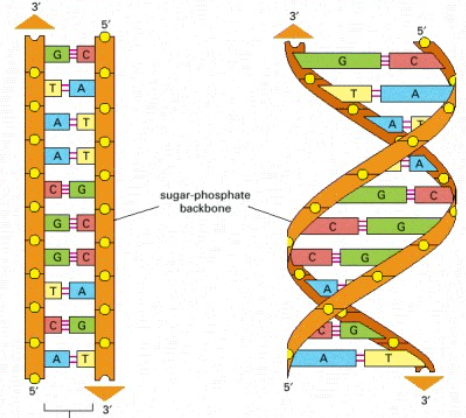
\includegraphics[width=0.5\textwidth]{images/dnk.png}
\caption{Struktura DNK  \cite{alberts2022}}
\label{fig:dnk}
\end{figure}

DNK je u ćelijama organizovana u strukture koje se nazivaju hromozomi. Skup svih DNK molekula jednog organizma, odnosno kompletna informacija sadržana u njegovim hromozomima, naziva se genom. Različiti organizmi imaju različit broj hromozoma, kao i genom različite dužine, koji može varirati od nekoliko stotina hiljada do više miliona nukleotida.

Sa stanovišta bioinformatike, DNK sekvenca se može predstaviti kao konačna niska karaktera nad alfabetom $\{A, C, G, T\}$. Podniske te niske, dužine $k$, nazivaju se $k$-grami i predstavljaju osnovne jedinice koje se analiziraju u bioinformatici. Analiza učestalosti i raspodele $k$-grama u genomu omogućava otkrivanje obrazaca koji mogu ukazivati na funkcionalno značajne regione DNK. Ovakav model omogućava primenu algoritamskih metoda za analizu sekvenci, prepoznavanje obrazaca i rešavanje različitih problema u obradi genetskih podataka.


\section{Replikacija DNK}
Replikacija DNK predstavlja proces umnožavanja genetskog materijala koji se odvija pre deobe ćelije. Tokom ovog procesa, dva lanca DNK se razdvajaju, a zatim se za svaki od njih sintetiše novi komplementarni lanac. Kao rezultat replikacije nastaju dve identične kopije originalnog DNK molekula, koje se raspodeljuju u ćerke ćelije. Slika \ref{fig:replication} ilustruje opisano.

\begin{figure}[h]
\centering
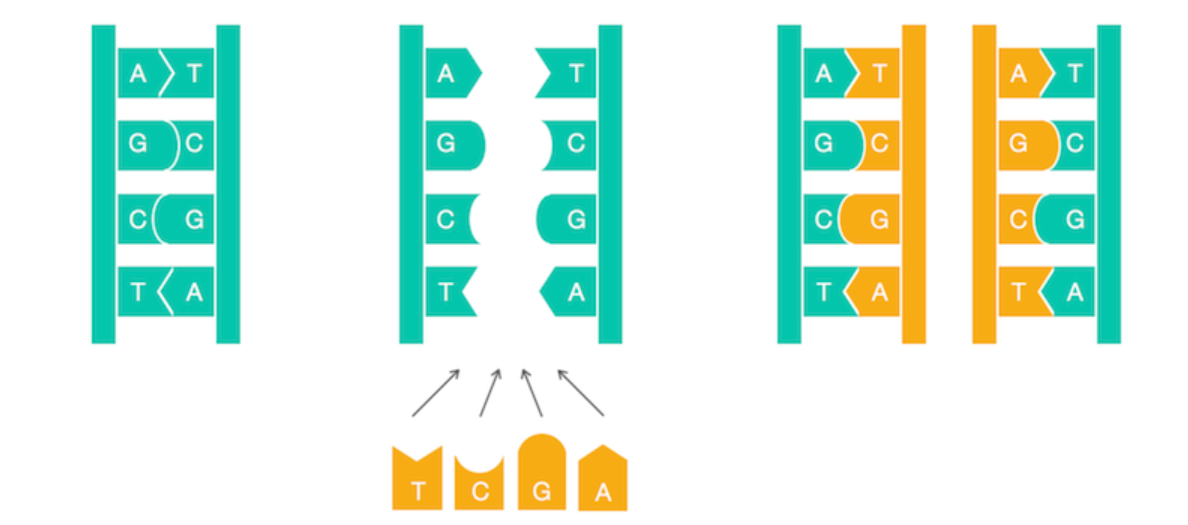
\includegraphics[width=0.7\textwidth]{images/replikacija.png}
\caption{Replikacija DNK\cite{online_book}}
\label{fig:replication}
\end{figure}
Ovaj proces je strogo regulisan, jer njegovo pokretanje i odvijanje kontrolišu različiti enzimi i drugi proteini kako bi replikacija započela na odgovarajućim lokacijama u genomu. Nakon toga, replikacija se odvija u oba smera duž DNK molekula, pri čemu dolazi do razdvajanja roditeljskih lanaca i sinteze novih komplementarnih nukleotidnih lanaca.

\section{Početni region replikacije (\textit{oriC})}
Početni region replikacije, označen kao \textit{oriC}, predstavlja specifičan segment DNK u kojem započinje proces replikacije. Kod bakterija, genom je najčešće organizovan u obliku kružnog hromozoma i sadrži samo jedan takav region iz kojeg se replikacija odvija u oba smera, kao što je prikazano na Slici \ref{fig:oric}.

\begin{figure}[h]
\centering
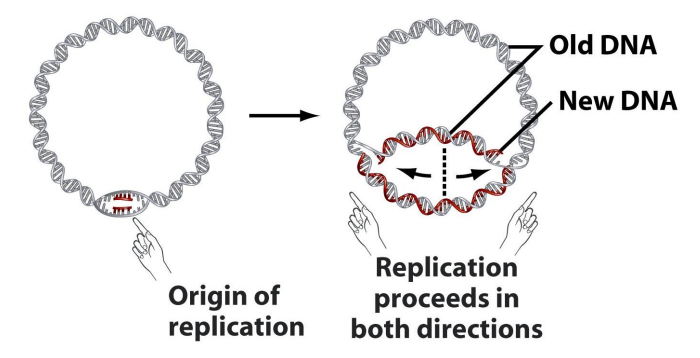
\includegraphics[width=0.7\textwidth]{images/oric.png}
\caption{Početni region replikacije \cite{online_lecture}}
\label{fig:oric}
\end{figure}
Ovaj region sadrži sekvence koje omogućavaju vezivanje proteina neophodnih za početak replikacije i time ima ključnu ulogu u pokretanju celokupnog procesa umnožavanja genetskog materijala. Iako je \textit{oriC} relativno kratak u poređenju sa dužinom celog genoma, koji može sadržati milione nukleotida, on u DNK sekvenci nije eksplicitno označen, odnosno ne postoji jedinstvena sekvenca ili oznaka koja direktno ukazuje na njegovu lokaciju. Zbog toga, njegovo pronalaženje predstavlja složen i netrivijalan zadatak.





\section{\textit{DNK} polimeraza, \textit{DnkA} proteini i boksovi}
Početak replikacije DNK započinje vezivanjem specifičnih proteina za određene delove genoma. Jedan od najvažnijih proteina u ovom procesu je \textit{DnkA}, koji ima sposobnost da prepozna i veže se za kratke sekvence unutar početnog regiona replikacije. Ove kratke sekvence poznate su kao \textit{DnkA} boksovi i karakteriše ih to što se pojavljuju više puta unutar \textit{oriC} regiona. Njihova učestalost na ograničenom regionu unutar DNK omogućava proteinima da identifikuju mesto na kojem treba da započne replikacija.
Nakon vezivanja \textit{DnkA} proteina dolazi do lokalnog razdvajanja DNK lanca, čime se omogućava delovanje \textit{DNK polimeraze}, enzima koji funkcioniše kao molekularna mašina za kopiranje genetskog materijala i vrši sintezu novih, komplementarnih DNK lanaca.
Upravo zbog svoje ponavljajuće prirode, \textit{DnkA} boksovi se mogu posmatrati kao karakteristični obrasci u DNK sekvenci, što omogućava njihovo pronalaženje primenom algoritamskih metoda. 




\section{Obrnuti komplement}

Zbog komplementarne prirode DNK molekula, svaki lanac DNK povezan je sa drugim lancem prema pravilima uparivanja baza, pri čemu se adenin (A) uparuje sa timinom (T), dok se guanin (G) uparuje sa citozinom (C). Pored toga, dva lanca DNK molekula imaju suprotnu orijentaciju (antiparalelni su), odnosno jedan je orijentisan u smeru $5' \rightarrow 3'$, a drugi u smeru $3' \rightarrow 5'$. Oznake $5'$ i $3'$ predstavljaju krajeve DNK lanca i određuju njegovu orijentaciju. Po konvenciji, DNK sekvence se zapisuju i čitaju u smeru $5' \rightarrow 3'$, što omogućava jednoznačno predstavljanje i poređenje sekvenci.

Na slici \ref{fig:reverse} prikazana su dva komplementarna DNK lanca i način uparivanja nukleotida. Može se uočiti da svakoj bazi jednog lanca odgovara tačno određena komplementarna baza na drugom lancu.

Na osnovu ovih osobina definiše se pojam obrnutog komplementa (eng. \textit{reverse complement}). Komplement jedne DNK sekvence dobija se zamenom svake baze njenom komplementarnom bazom. Zbog suprotne orijentacije DNK lanaca, komplementarna sekvenca čita se u smeru $5' \rightarrow 3'$, čime se dobija obrnuti komplement.

\begin{figure}[h]
\centering
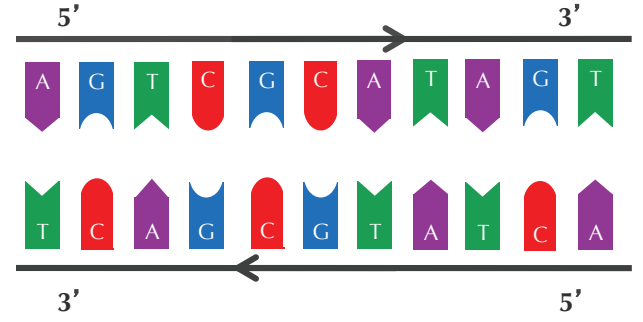
\includegraphics[width=0.7\textwidth]{images/reverse.png}
\caption{Komplementarni DNK lanci i suprotna orijentacija lanaca \cite{online_book}}
\label{fig:reverse}
\end{figure}

Na primer, za sekvencu \code{AGTC}, komplementarna sekvenca je \code{TCAG}, dok je njen obrnuti komplement \code{GACT}.



S obzirom na dvostruku strukturu DNK molekula, biološki značajne sekvence mogu se pojaviti na bilo kom od njegova dva lanca. Zbog toga je pri analizi genoma neophodno uzeti u obzir oba lanca DNK molekula. Kako se DNK sekvence po konvenciji zapisuju u smeru $5' \rightarrow 3'$, drugi lanac predstavlja se njegovim obrnutim komplementom. Ovo je od posebnog značaja u algoritmima za pronalaženje početnog regiona replikacije, jer omogućava prepoznavanje karakterističnih obrazaca bez obzira na lanac na kojem se nalaze.



% ------------------------------------------------------------------------------
\chapter{Algoritamski pristupi za pronalaženje početnog regiona replikacije}
% ------------------------------------------------------------------------------

Biološke osobine početnog regiona replikacije, kao što su prisustvo ponavljajućih sekvenci i statističke nepravilnosti u raspodeli nukleotida, omogućavaju primenu algoritamskih metoda za njegovo pronalaženje. Analizom učestalosti podniski, njihove lokalne raspodele i statističkih karakteristika genoma moguće je identifikovati potencijalne kandidate za \textit{oriC} region. U ovom poglavlju biće predstavljeni algoritamski pristupi koji koriste ove osobine za analizu DNK sekvenci.

\section{Problem čestih reči}

Kako određeni obrasci u DNK sekvenci mogu ukazivati na funkcionalno važne regione, prirodan pristup jeste analiza učestalosti pojavljivanja podniski. Sekvence koje se pojavljuju značajno češće od ostalih mogu imati posebnu biološku ulogu, pa se problem svodi na pronalaženje najčešće zastupljenih podniski određene dužine.

Polazeći od pretpostavke da se DNK sekvenca može posmatrati kao niska karaktera nad alfabetom $\{A, C, G, T\}$, moguće je primeniti metode analize teksta u cilju identifikacije karakterističnih obrazaca.

Podniske dužine $k$ jedne biološke sekvence (DNK, njenog segmenta ili proteina) nazivaju se $k$-grami (eng.\textit{ $k$-mers}) i predstavljaju osnovne jedinice analize bioloških sekvenci. Analizom njihovog broja pojavljivanja moguće je identifikovati obrasce koji mogu ukazivati na prisustvo funkcionalno značajnih regiona, kao što je \textit{oriC}. 

Neka je data niska $Text$ i podniska $Pattern$ dužine $k$.  Definišemo funkciju:
\[
\textit{PatternCount}(Text, Pattern)
\]
kao broj pojavljivanja podniske $Pattern$ u niski $Text$, pri čemu se uzimaju u obzir i preklapajuća pojavljivanja.

\subsubsection{Algoritam za prebrojavanje pojavljivanja}

Za izračunavanje funkcije $\textit{PatternCount}(Text, Pattern)$ koristi se pristup zasnovan na kliznom prozoru (eng. \textit{sliding window}). Ideja je da se prolaskom kroz tekst proveri svaka podniska dužine $k$.

Algoritam \ref{alg:pattern_count} prikazuje pseudokod za izračunavanje ove funkcije.

\begin{algorithm}[h]
\caption{Pattern Count}
\label{alg:pattern_count}
\SetAlgoLined
\DontPrintSemicolon
\SetKwFunction{FRec}{PatternCount}
\SetKwProg{Fn}{Funkcija}{}{}
\Fn{\FRec{Text, Pattern}}{
    $count \gets 0$\;

    \For{$i \gets 0$ \KwTo $|Text| - |Pattern|$}{
        \If{$Text[i\,..\,(i+|Pattern|-1)] = Pattern$}{
            $count \gets count + 1$\;
        }
    }

    \Return{$count$}
}
\end{algorithm}

\subsection{Algoritam}

Problem čestih reči (eng. \textit{Frequent Words Problem}) može se formalno definisati na sledeći način:

\begin{itemize}
    \item Ulaz: niska karaktera $Text$ i ceo broj $k$
    \item Izlaz: skup svih $k$-grama koji maksimizuju $\textit{PatternCount}(Text, Pattern)$
\end{itemize}

Kažemo da je $k$-gram najčešći ukoliko se nijedan drugi $k$-gram ne pojavljuje više puta od njega u posmatranoj sekvenci.



\subsubsection{Ideja i opis algoritma}

Osnovna ideja algoritma za pronalazak čestih reči zasniva se na prolasku kroz celu DNK sekvencu i prebrojavanju koliko puta se svaka podniska dužine $k$ pojavljuje. Nakon toga se izdvajaju one podniske koje se pojavljuju maksimalan broj puta.

Naivni pristup rešavanju ovog problema može se opisati kroz sledeće korake:
\begin{itemize}
    \item Proći kroz sve moguće pozicije u niski $Text$.
    \item Za svaku moguću početnu poziciju u niski izdvojiti podnisku dužine $k$ koja počinje na toj poziciji.
    \item Za svaku podnisku izračunati $\textit{PatternCount}(Text, Pattern)$ primenom algoritma \ref{alg:pattern_count}.
    \item Odrediti maksimalan broj pojavljivanja.
    \item Izdvojiti sve podniske koje imaju tu frekvenciju.
\end{itemize}

Algoritam \ref{alg:frequent_words} prikazuje pseudokod algoritma za pronalaženje najčešćih reči.

\begin{algorithm}[h]
\caption{Frequent Words}
\label{alg:frequent_words}
\SetAlgoLined
\DontPrintSemicolon
\SetKwFunction{FRec}{FrequentWords}
\SetKwProg{Fn}{Funkcija}{}{}
\Fn{\FRec{Text, k}}{
    $najcesciKgrami \gets$ prazan skup\;
    $count \gets$ niz dužine $|Text|-k+1$ inicijalizovan nulama\;

    \For{$i \gets 0$ \KwTo $|Text| - k$}{
        $pattern \gets Text[i..i+k-1]$\;
        $count[i] \gets$ PatternCount$(Text, pattern)$\;
    }

    $maxBroj \gets$ maksimalna vrednost u nizu $count$\;

    \For{$i \gets 0$ \KwTo $|Text| - k$}{
        \If{$count[i] = maxBroj$}{
            dodaj $Text[i..i+k-1]$ u $najcesciKgrami$\;
        }
    }

    ukloni duplikate iz $najcesciKgrami$\;

    \Return{$najcesciKgrami$}
}
\end{algorithm}



\subsubsection{Primer}

Posmatrajmo DNK sekvencu:
\[
\texttt{ACTGACTCCCACCCC}
\]

Za $k = 3$ izdvajaju se svi 3-grami i računa se broj njihovih pojavljivanja u sekvenci.

Neki od izdvojenih 3-grama su:
\[
\texttt{ACT},\ \texttt{CTG},\ \texttt{TGA},\ \texttt{GAC},\ \texttt{ACT},\ \dots
\]

Algoritam \textit{\textbf{PatternCount}} za svaki obrazac prolazi kroz celu sekvencu i određuje koliko puta se dati 3-gram pojavljuje. Važno je napomenuti da algoritam \textit{\textbf{PatternCount}} uzima u obzir i preklapajuća pojavljivanja podniski. To znači da nova pojava podniske može započeti pre nego što se prethodna potpuno završi.

Na primer, u nizu:
\[
\texttt{ATATATA}
\]
podniska \texttt{ATA} pojavljuje se na pozicijama 0, 2 i 4, pri čemu se ova pojavljivanja međusobno preklapaju.

Primenom algoritma \textit{\textbf{PatternCount}} za svaki izdvojeni 3-gram računa se broj njegovih pojavljivanja u celoj sekvenci. Na slici \ref{figg:count} prikazan je niz \textit{\textbf{Count}} kreiran primenom algoritma \ref{alg:frequent_words}.

\begin{figure}[h]
\centering

\includegraphics[width=0.75\textwidth]{images/count_ex.png}
\caption{Primer izdvajanja 3-grama i određivanja njihovih frekvencija \cite{online_book}.}
\label{figg:count}
\end{figure}
Na primer:
\[
\text{PatternCount}(\texttt{Text}, \texttt{ACT}) = 2
\]

jer se obrazac \texttt{ACT} pojavljuje dva puta u sekvenci.

Slično tome:
\[
\text{PatternCount}(\texttt{Text}, \texttt{CCC}) = 3
\]

što znači da je \texttt{CCC} najčešći 3-gram u datoj sekvenci.


\subsection{Vremenska složenost}

Algoritam \textit{\textbf{PatternCount}} prolazi kroz sve moguće pozicije u niski $Text$, kojih ima $|Text| - k + 1$. Za svaku poziciju vrši se poređenje podniske dužine $k$, što zahteva do $k$ poređenja karaktera. Zbog toga je vremenska složenost ovog algoritma:

\[
O((|Text| - k + 1) \cdot k)
\]

što se za velike vrednosti $|Text|$ može aproksimirati kao:

\[
O(|Text| \cdot k)
\]

Algoritam \textit{\textbf{FrequentWords}} generiše $|Text| - k + 1$ $k$-grama i za svaki od njih poziva funkciju \textit{\textbf{PatternCount}}. Stoga je ukupan broj operacija:

\[
(|Text| - k + 1) \cdot ((|Text| - k + 1) \cdot k)
\]

što daje ukupnu vremensku složenost:

\[
O((|Text| - k + 1)^2 \cdot k)
\]

Za velike vrednosti ulaza, ova složenost se može pojednostaviti na:

\[
O(|Text|^2 \cdot k)
\]

Drugim rečima, algoritam ima kvadratnu složenost u odnosu na dužinu sekvence, uz dodatni faktor $k$ koji odgovara dužini analiziranih podniski.

Ovakva složenost brzo postaje nepraktična za duge DNK sekvence, koje mogu sadržati milione nukleotida. Zbog toga je neophodno razmotriti optimizovane pristupe, poput korišćenja niza frekvencija ili sortiranja, koji omogućavaju značajno efikasnije rešavanje ovog problema. Ovi pristupi biće detaljno analizirani u sekcijama \ref{sec:niz_frekvencija} i  \ref{sec:sortiranje}.


\subsection{Optimizovani pristup korišćenjem niza frekvencija}
\label{sec:niz_frekvencija}
Naivni algoritam za rešavanje problema čestih reči ima visoku vrsemensku složenost jer za svaki $k$-gram ponovo prolazi kroz celu sekvencu. Da bi se ovaj problem rešio efikasnije, uvodi se optimizovani pristup zasnovan na korišćenju niza frekvencija.

Osnovna ideja je da se kroz sekvencu prolazi samo jednom, pri čemu se za svaki $k$-gram beleži broj njegovih pojavljivanja. Umesto ponovnog prebrojavanja, rezultati se čuvaju u strukturi podataka koja omogućava brz pristup.


\subsubsection{Leksikografsko indeksiranje i numerička reprezentacija $k$-grama}

Kako bi se omogućilo efikasno skladištenje i pretraživanje, svaki $k$-gram se mapira na jedinstveni indeks. S obzirom na to da DNK alfabet sadrži četiri simbola, postoji ukupno $4^k$ mogućih $k$-grama.

Ovi $k$-grami se mogu poređati leksikografski (kao u rečniku), pri čemu se svakom dodeljuje jedinstveni broj iz opsega $[0, 4^k - 1]$.

Za ovu transformaciju koriste se funkcije \textit{\textbf{PatternToNumber}} i \textit{\textbf{NumberToPattern}}, koje omogućavaju prelazak između simboličke i numeričke reprezentacije $k$-grama.

DNK alfabet $\{A, C, G, T\}$  može se mapirati na sledeći:
\[
A \rightarrow 0,\quad C \rightarrow 1,\quad G \rightarrow 2,\quad T \rightarrow 3
\]


Funkcija \textit{\textbf{SymbolToNumber}} predstavlja pomoćnu funkciju koja svakom simbolu DNK alfabeta (\texttt{A}, \texttt{C}, \texttt{G}, \texttt{T}) dodeljuje odgovarajuću numeričku vrednost (\texttt{0}, \texttt{1}, \texttt{2}, \texttt{3}), čime omogućava numeričku reprezentaciju $k$-grama u sistemu sa osnovom 4.

Funkcija \textit{\textbf{PatternToNumber}} preslikava dati k-gram u odgovarajući broj koristeći zapis u brojnom sistemu sa osnovom 4. Pri tome se prefiks k-grama posmatra kao već izračunata vrednost, koja se množi sa 4 i uvećava za numeričku vrednost poslednjeg simbola. Ovaj postupak odgovara standardnoj konverziji iz pozicionog brojnog sistema i i omogućava da se svaki k-gram jednoznačno predstavi celobrojnom vrednošću. U algoritmu zasnovanom na nizu frekvencija, dobijena celobrojna vrednost predstavlja indeks odgovarajućeg elementa niza frekvencija, u kojem se čuva broj pojavljivanja datog k-grama. Algoritam \ref{alg:pattern_to_number} prikazuje pseudokod  funkcije \textit{\textbf{PatternToNumber}}.

\begin{algorithm}[h]
\caption{PatternToNumber}
\label{alg:pattern_to_number}
\SetAlgoLined
\DontPrintSemicolon
\SetKwFunction{FRec}{PatternToNumber}
\SetKwProg{Fn}{Funkcija}{}{}
\Fn{\FRec{Pattern}}{
\If{$Pattern$ je prazan}{
    \Return{$0$}
}

$symbol \gets$ poslednji simbol u $Pattern$\;
$prefix \gets$ $Pattern$ bez poslednjeg simbola\;

\Return{$4 \cdot$ PatternToNumber$(prefix)$ $+$ SymbolToNumber$(symbol)$}
}
\end{algorithm}

Obrnuta transformacija vrši se funkcijom \textit{\textbf{NumberToPattern}}, koja dati indeks pretvara nazad u odgovarajući $k$-gram. Funkcija \textit{\textbf{NumberToSymbol}} vrši obrnutu transformaciju u odnosu na funkciju \textit{\textbf{SymbolToNumber}}, tako što svakoj numeričkoj vrednosti iz skupa \texttt{(0,1,2,3)} dodeljuje odgovarajući simbol DNK alfabeta (\texttt{A}, \texttt{C}, \texttt{G}, \texttt{T}). Algoritam \ref{alg:number_to_pattern} prikazuje pseudokod funkcije \textit{\textbf{NumberToSymbol}}, koriste se operacije celobrojnog deljenja i ostatka pri deljenju sa 4: količnik određuje prefiks, dok ostatak određuje poslednji simbol. Na taj način se postupno rekonstruiše ceo $k$-gram. 

\begin{algorithm}[h]
\caption{NumberToPattern}
\label{alg:number_to_pattern}
\SetAlgoLined
\DontPrintSemicolon
\SetKwFunction{FRec}{NumberToPattern}
\SetKwProg{Fn}{Funkcija}{}{}
\Fn{\FRec{index, k}}{
\If{$k = 1$}{
    \Return NumberToSymbol$(index)$
}

$prefixIndex \gets \lfloor index / 4 \rfloor$\;
$r \gets index \bmod 4$\;
$symbol \gets$ NumberToSymbol$(r)$\;

$prefixPattern \gets$ NumberToPattern$(prefixIndex, k-1)$\;

\Return konkatenacija $prefixPattern$ i $symbol$
}
\end{algorithm}

Ove dve funkcije zajedno omogućavaju efikasan prelazak između simboličke i numeričke reprezentacije $k$-grama, što je ključno za implementaciju algoritama zasnovanih na nizovima frekvencija.



\subsubsection{Algoritam}

Algoritam za izračunavanje frekvencija prolazi kroz tekst samo jednom i za svaki $k$-gram povećava odgovarajući element niza frekvencija. Pseudokod prikazuje Algoritam \ref{alg:computing_frequencies}.

\begin{algorithm}[h]
\caption{Computing Frequencies}
\label{alg:computing_frequencies}
\SetAlgoLined
\DontPrintSemicolon
\SetKwFunction{FRec}{ComputingFrequencies}
\SetKwProg{Fn}{Funkcija}{}{}
\Fn{\FRec{Text, k}}{
\For{$i \gets 0$ \KwTo $4^k - 1$}{
    $FrequencyArray[i] \gets 0$\;
}

\For{$i \gets 0$ \KwTo $|Text| - k$}{
    $Pattern \gets Text[i..i+k-1]$\;
    $j \gets PatternToNumber(Pattern)$\;
    $FrequencyArray[j] \gets FrequencyArray[j] + 1$\;
}

\Return{$FrequencyArray$}
}
\end{algorithm}



Nakon što je niz frekvencija izračunat, najčešći $k$-grami se dobijaju pronalaženjem maksimalne vrednosti u nizu i identifikacijom svih indeksa i njima odgovarajućih k-grama koji imaju tu vrednost. Algoritam \ref{alg:faster_frequent_words} prikazuje pseudokod funkcije \textit{Faster Frequent Words}.


\begin{algorithm}[h]
\caption{Faster Frequent Words}
\label{alg:faster_frequent_words}
\SetAlgoLined
\DontPrintSemicolon
\SetKwFunction{FRec}{FasterFrequentWords}
\SetKwProg{Fn}{Funkcija}{}{}
\Fn{\FRec{Text, k}}{
 $najcesciKgrami \gets$ prazan skup\;
$FrequencyArray \gets$ ComputingFrequencies$(Text, k)$\;
$maxCount \gets$ maksimalna vrednost u $FrequencyArray$\;

\For{$i \gets 0$ \KwTo $4^k - 1$}{
    \If{$FrequencyArray[i] = maxCount$}{
        $Pattern \gets$ NumberToPattern$(i, k)$\;
        dodaj $Pattern$ u skup rezultata\;
    }
}

\Return{$najcesciKgrami$}
}
\end{algorithm}


\subsubsection{Primer}

Za slučaj $k = 2$ postoji ukupno $4^2 = 16$ mogućih 2-grama. Oni se mogu poređati leksikografski, pri čemu svaki 2-gram dobija jedinstveni indeks iz opsega od 0 do 15.

Na slici \ref{fig:frequency} prikazan je primer leksikografskog uređenja svih mogućih 2-grama, zajedno sa odgovarajućim indeksima i nizom frekvencija za posmatranu DNK sekvencu.

Na primer, 2-gram \texttt{GT} ima indeks \texttt{11} što znači da funkcija: \textit{\texttt{PatternToNumber(GT)}}=11. Obrnuto, funkcija: \textit{\texttt{NumberToPattern}}(11,2) vraća \texttt{GT}.


Na ovaj način omogućava se efikasno mapiranje između simboličke i numeričke reprezentacije $k$-grama, što predstavlja osnovu za konstrukciju niza frekvencija. 

Niz frekvencija prikazan na Slici \ref{fig:frequency} predstavlja broj pojavljivanja svakog 2-grama u posmatranoj sekvenci. Na primer, vrednost 3 na poziciji koja odgovara 2-gramu \texttt{AA} pokazuje da se ovaj obrazac pojavljuje tri puta u sekvenci. Slično tome, 2-gram \texttt{GG} takođe ima frekvenciju 3, dok se neki obrasci ne pojavljuju nijednom, pa je njihova frekvencija jednaka 0. Na ovaj način niz frekvencija omogućava efikasno određivanje najčešćih $k$-grama bez ponovnog prolaska kroz celu sekvencu.

\begin{figure}[h]
\centering
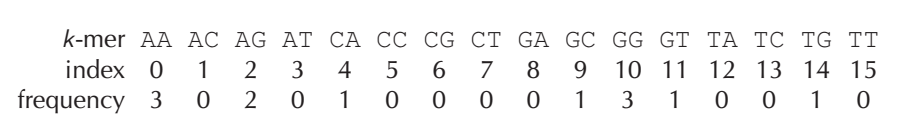
\includegraphics[width=0.8\textwidth]{images/frequency_array.png}
\caption{Leksikografsko indeksiranje 2-grama i primer niza frekvencija \cite{online_book}.}
\label{fig:frequency}
\end{figure}

\subsubsection{Vremenska složenost optimizovanog pristupa}

U ovom pristupu niska \textit{Text} se obrađuje samo jednom, pri čemu se za svaki $k$-gram vrši njegova obrada i konverzija u numerički oblik, što daje složenost $O(|Text| \cdot k)$.

Međutim, dodatni trošak predstavlja inicijalizacija niza frekvencija dimenzije $4^k$, kao i iteracija kroz ceo niz prilikom traženja maksimuma i rekonstrukcije odgovarajućih $k$-grama. Ukupna složenost algoritma iznosi:

\[
O(|Text| \cdot k + 4^k \cdot k)
\]

Za male vrednosti $k$, izraz $4^k$ može se smatrati konstantom, pa složenost postaje približno linearna u odnosu na dužinu teksta.

Prostorna složenost ovog pristupa određena je dimenzijom niza frekvencija, koji sadrži $4^k$ elemenata. Zbog toga prostorna složenost iznosi:

\[
O(4^k)
\]

Ovaj pristup je značajno efikasniji od naivnog algoritma kada je $k$ relativno malo u odnosu na $|Text|$. Međutim, zbog eksponencijalnog rasta izraza $4^k$, ovaj metod postaje nepraktičan za veće vrednosti $k$, što motiviše razvoj dodatnih optimizacija.

\subsection{Optimizovani pristup korišćenjem heš mape}

Prethodno opisani pristup korišćenjem niza frekvencija omogućava efikasnije rešavanje problema čestih reči u odnosu na naivni algoritam, ali ima jedan važan nedostatak. Dimenzija niza frekvencija iznosi $4^k$, jer se unapred rezerviše mesto za svaki mogući $k$-gram nad DNK alfabetom. Kada je vrednost $k$ veća, broj mogućih $k$-grama raste eksponencijalno, pa ovaj pristup može zahtevati veliku količinu memorije.

Da bi se ovaj problem ublažio, uvodi se optimizovani pristup zasnovan na korišćenju heš mape, odnosno rečnika. Umesto da se čuva frekvencija za svaki mogući $k$-gram, u memoriji se čuvaju samo brojači onih $k$-grama koji se zaista pojavljuju u posmatranoj DNK sekvenci.

Osnovna ideja je ista kao u prethodno objašnjenom pristupu, odnosno, kroz nisku \textit{Text} prolazi se samo jednom. U svakom koraku izdvaja se trenutni $k$-gram, a zatim se u heš mapi ažurira broj njegovih pojavljivanja. Ključ u heš mapi predstavlja $k$-gram, dok vrednost predstavlja broj njegovih pojavljivanja u tekstu.

Ako se posmatrani $k$-gram prvi put pojavljuje, on se dodaje u heš mapu sa vrednošću 1. Ukoliko već postoji u heš mapi, njegova vrednost se uvećava za 1. Na taj način se izbegava ponovno prebrojavanje pojavljivanja istog k-grama, kao i čuvanje frekvencija za k-grame koji se uopšte ne pojavljuju u sekvenci.

\subsubsection{Algoritam}

Algoritam za izračunavanje frekvencija pomoću heš mape prolazi kroz tekst i za svaki pronađeni $k$-gram ažurira odgovarajuću vrednost u rečniku. Pseudokod je prikazan u Algoritmu \ref{alg:computing_frequencies_with_dictionary}.

\begin{algorithm}[h]
\caption{Computing Frequencies With Dictionary}
\label{alg:computing_frequencies_with_dictionary}
\SetAlgoLined
\DontPrintSemicolon
\SetKwFunction{FRec}{ComputingFrequenciesWithDictionary}
\SetKwProg{Fn}{Funkcija}{}{}
\Fn{\FRec{Text, k}}{
$FrequencyMap \gets$ prazna heš mapa\;

\For{$i \gets 0$ \KwTo $|Text| - k$}{
    $Pattern \gets Text[i..i+k-1]$\;

    \If{$Pattern$ nije ključ u $FrequencyMap$}{
        $FrequencyMap[Pattern] \gets 1$\;
    }
    \Else{
        $FrequencyMap[Pattern] \gets FrequencyMap[Pattern] + 1$\;
    }
}

\Return{$FrequencyMap$}
}
\end{algorithm}

Nakon što su frekvencije svih pronađenih $k$-grama izračunate, najčešći $k$-grami se dobijaju pronalaženjem maksimalne vrednosti u heš mapi. Kao što je prikazano u Algoritmu \ref{alg:faster_frequent_words_d}, svi obrasci čija je vrednost jednaka maksimumu dodaju se u skup rezultata \cite{matf_repo}.  

\begin{algorithm}[h]
\caption{Faster Frequent Words With Dictionary}
\label{alg:faster_frequent_words_d}
\SetAlgoLined
\DontPrintSemicolon
\SetKwFunction{FRec}{FasterFrequentWordsWithDictionary}
\SetKwProg{Fn}{Funkcija}{}{}
\Fn{\FRec{Text, k}}{
$FrequentPatterns \gets$ prazan skup\;
$FrequencyMap \gets$ ComputingFrequenciesWithDictionary$(Text, k)$\;
$maxCount \gets$ maksimalna vrednost u $FrequencyMap$\;

\ForEach{$Pattern$ u $FrequencyMap$}{
    \If{$FrequencyMap[Pattern] = maxCount$}{
        dodaj $Pattern$ u $FrequentPatterns$\;
    }
}

\Return{$FrequentPatterns$}
}
\end{algorithm}

\subsubsection{Primer}

Neka je data DNK sekvenca \texttt{ACTGACTCCCACCCC} i neka je $k = 3$. Algoritam posmatra sve 3-grame koji se pojavljuju u tekstu pomeranjem prozora dužine 3 za jedno mesto udesno.

Na početku je heš mapa prazna. Prvi posmatrani 3-gram je \texttt{ACT}, pa se on dodaje u heš mapu sa vrednošću 1. Zatim se posmatra 3-gram \texttt{CTG}, koji se takođe dodaje sa vrednošću 1. Kada se kasnije ponovo pojavi 3-gram \texttt{ACT}, njegova vrednost u heš mapi se uvećava sa 1 na 2.

Na ovaj način heš mapa postepeno beleži broj pojavljivanja svakog 3-grama koji se zaista javlja u sekvenci. Na kraju obrade, najčešći 3-gram je onaj čija je vrednost u heš mapi najveća. Ako više različitih 3-grama ima istu maksimalnu vrednost, svi oni predstavljaju rezultat problema čestih reči.


\subsubsection{Vremenska složenost optimizovanog pristupa korišćenjem heš mape}

U ovom pristupu tekst se obrađuje samo jednom, pri čemu se u svakom koraku izdvaja jedan $k$-gram i ažurira njegova vrednost u heš mapi. Izdvajanje podniske dužine $k$ zahteva $O(k)$ operacija, dok je pristup i ažuriranje vrednosti u heš mapi u prosečnom slučaju $O(1)$.

S obzirom na to da se ova operacija izvršava za svih $|Text| - k + 1$ pozicija, ukupna složenost ove faze iznosi:

\[
O(|Text| \cdot k)
\]

Nakon toga, potrebno je pronaći maksimalnu vrednost u heš mapi, što zahteva prolazak kroz sve njene elemente. U najgorem slučaju, broj različitih $k$-grama je najviše $|Text| - k + 1$, pa je za ovaj korak potrebno:

\[
O(|Text|)
\]

Kombinovanjem svih koraka dolazi se do ukupne vremenske složenosti:

\[
O(|Text| \cdot k)
\]

Za razliku od pristupa sa nizom frekvencija, ovde nije potrebno inicijalizovati niz dimenzije $4^k$, niti prolaziti kroz sve moguće $k$-grame. Pretražuju se samo oni obrasci koji su se stvarno pojavili u niski \textit{Text}.

Prostorna složenost zavisi od broja različitih $k$-grama u posmatranoj sekvenci. U najgorem slučaju, svi izdvojeni $k$-grami mogu biti različiti, pa je broj elemenata u heš mapi najviše $|Text| - k + 1$. Kako svaki $k$-gram zauzima $O(k)$ memorije, ukupna prostorna složenost iznosi:

\[
O(|Text| \cdot k)
\]

Ovaj pristup je posebno koristan za veće vrednosti $k$, jer izbegava eksponencijalni memorijski trošak koji nastaje kod niza frekvencija. Zbog toga predstavlja efikasniju optimizaciju kada nije potrebno čuvati informacije o $k$-gramima koji se ne pojavljuju u ulaznoj sekvenci.

\subsection{Pronalaženje najčešćih $k$-grama sortiranjem}
\label{sec:sortiranje}
Pored pristupa zasnovanog na nizu frekvencija, problem čestih reči može se rešiti i korišćenjem sortiranja. Osnovna ideja ovog pristupa je da se svi $k$-grami najpre transformišu u numeričke vrednosti, nakon čega se sortiraju, čime se identični elementi grupišu jedan do drugog.

Neka je data niska $Text$. Za svaku poziciju $i$ izdvajamo $k$-gram $Text[i..i+k-1]$ i transformišemo ga u odgovarajući broj korišćenjem funkcije \textit{\textbf{PatternToNumber}}. Na taj način dobijamo niz indeksa koji zatim sortiramo. 

Nakon sortiranja, identični $k$-grami se pojavljuju u uzastopnim segmentima niza, što omogućava jednostavno prebrojavanje njihovih pojavljivanja. Algoritam \ref{alg:ffw_sorting} prikazuje pseudokod ovog pristupa.

\begin{algorithm}[h]
\caption{Finding Frequent Words by Sorting}
\label{alg:ffw_sorting}
\SetAlgoLined
\DontPrintSemicolon
\SetKwFunction{FRec}{FindingFrequentWordsBySorting}
\SetKwProg{Fn}{Funkcija}{}{}
\Fn{\FRec{Text, k}}{
$FrequentPatterns \gets$ prazan skup\;

\For{$i \gets 0$ \KwTo $|Text|-k$}{
    $Pattern \gets Text[i..i+k-1]$\;
    $Index[i] \gets$ PatternToNumber$(Pattern)$\;
    $Count[i] \gets 1$\;
}

$SortedIndex \gets$ Sort$(Index)$\;

\For{$i \gets 1$ \KwTo $|Text|-k$}{
    \If{$SortedIndex[i] = SortedIndex[i-1]$}{
        $Count[i] \gets Count[i-1] + 1$\;
    }
}

$maxCount \gets$ maksimalna vrednost u $Count$\;

\For{$i \gets 0$ \KwTo $|Text|-k$}{
    \If{$Count[i] = maxCount$}{
        $Pattern \gets$ NumberToPattern$(SortedIndex[i], k)$\;
        dodaj $Pattern$ u $FrequentPatterns$\;
    }
}

\Return{$FrequentPatterns$}
}
\end{algorithm}
\subsubsection{Primer}

Posmatrajmo DNK sekvencu:
\[
\texttt{AAGCAAAGGTGGG}
\]

Za $k = 2$ izdvajaju se svi 2-grami redom kojim se pojavljuju u sekvenci i transformišu se u odgovarajući numerički indeks korišćenjem funkcije \textit{\textbf{PatternToNumber}}. Na taj način dobija se niz prikazan na Slici \ref{fig:sorting}.
\begin{figure}[h]
\centering
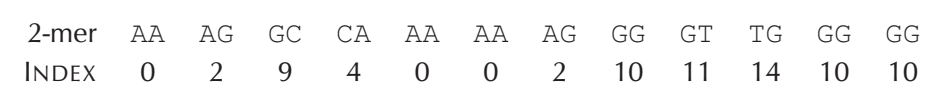
\includegraphics[width=0.8\textwidth]{images/sorting.png}
\caption{Izdvajanje i transformacija 2-grama \cite{online_book}.}
\label{fig:sorting}
\end{figure}


Nakon sortiranja identični indeksi se grupišu jedan do drugog (Slika \ref{fig:sorted}). Zatim se prolaskom kroz sortirani niz određuje dužina svakog uzastopnog segmenta identičnih indeksa. Segment sa najvećim brojem elemenata odgovara k-gramu koji se pojavljuje najveći broj puta u posmatranoj sekvenci.

\begin{figure}[h]
\centering

\includegraphics[width=0.8\textwidth]{images/sorted.png}
\caption{Primer sortiranja indeksa i grupisanja identičnih $k$-grama \cite{online_book}.}
\label{fig:sorted}
\end{figure}



U ovom primeru indeks \texttt{0} odgovara 2-gramu \texttt{AA}, dok indeks \texttt{10} odgovara 2-gramu \texttt{GG}. Kako se oba indeksa pojavljuju tri puta, zaključuje se da su \texttt{AA} i \texttt{GG} najčešći 2-grami u datoj sekvenci.





\subsubsection{Vremenska složenost pristupa zasnovanog na sortiranju}

U ovom pristupu generiše se niz od $|Text| - k + 1$ elemenata, nakon čega se vrši sortiranje tog niza. Dominantna operacija je sortiranje, čija složenost iznosi:

\[
O(|Text| \log |Text|)
\]

Dodatne operacije, poput transformacije $k$-grama i prolaska kroz niz, imaju složenost $O(|Text| \cdot k)$.

Ukupna vremenska složenost algoritma je:

\[
O(|Text| \log |Text| + |Text| \cdot k)
\]

\subsection{Poređenje različitih pristupa}


Na osnovu poređenja prikazanog u Tabeli \ref{tab:comparison} može se zaključiti da izbor algoritma zavisi od vrednosti parametra $k$, dužine ulazne sekvence \textit{Text} i raspoloživih memorijskih resursa. Pristup zasnovan na nizu frekvencija efikasan je za manje vrednosti parametra $k$, dok je za veće vrednosti pogodniji pristup zasnovan na heš mapi, jer ne zahteva memoriju veličine $4^k$. Pristup zasnovan na sortiranju predstavlja kompromis između vremenske i prostorne složenosti, dok je naivni algoritam prvenstveno pogodan za ilustraciju problema i obradu kraćih sekvenci.
\begin{table}[H]
\centering
\renewcommand{\arraystretch}{1}
\begin{tabular}{|>{\raggedright\arraybackslash}m{0.28\textwidth}|>{\centering\arraybackslash}m{0.24\textwidth}|>{\centering\arraybackslash}m{0.20\textwidth}|>{\raggedright\arraybackslash}m{0.20\textwidth}|}
\hline
\textbf{Pristup} & \textbf{Vremenska složenost} & \textbf{Prostorna složenost} & \textbf{Karakteristike} \\
\hline
Naivni algoritam &
$O(|Text|^2 \cdot k)$ &
$O(|Text|)$ &
Jednostavna implementacija, ali veoma spor za duže sekvence. \\
\hline

Niz frekvencija &
$O(|Text|\cdot k + 4^k \cdot k)$ &
$O(4^k)$ &
Efikasan za male vrednosti $k$, ali zahteva memoriju veličine $4^k$. \\
\hline

Heš mapa &
$O(|Text|\cdot k)$ &
$O(|Text|\cdot k)$ &
Čuvaju se samo $k$-grami koji se pojavljuju u sekvenci. \\
\hline

Sortiranje &
$O(|Text|\log|Text| + |Text|\cdot k)$ &
$O(|Text|)$ &
Ne zahteva niz veličine $4^k$, ali je sporiji od pristupa sa heš mapom zbog sortiranja. \\
\hline
\end{tabular}
\caption{Poređenje različitih pristupa za rešavanje problema čestih reči}
\label{tab:comparison}
\end{table}


\section{Problem pronalaženja grupa}

Sama učestalost podniski na nivou celog genoma nije uvek dovoljna za preciznu identifikaciju funkcionalno značajnih regiona. U praksi je često mnogo značajnije posmatrati lokalnu frekvenciju podniski unutar kraćih segmenata genoma. Na primer, određeni $k$-gram može se pojavljivati relativno često u celom genomu, ali ukoliko su njegova pojavljivanja grupisana u kratkom regionu, takav obrazac može ukazivati na biološki značajan signal. Ovakva pojava je posebno izražena kod \textit{DnkA} boksova, koji se često pojavljuju u grupama unutar početnog regiona replikacije, odnosno \textit{oriC} regiona. Zbog toga analiza lokalnih ponavljanja predstavlja prirodno proširenje problema čestih reči.

\subsubsection{Motivacija i veza sa biološkim problemom}

Nakon identifikacije čestih obrazaca u poznatim \textit{oriC} regionima, postavlja se ključno pitanje: kako pronaći slične regione u genomu kada početni region replikacije nije unapred poznat? U takvoj situaciji nije dovoljno posmatrati samo globalno najčešće $k$-grame, jer se biološki relevantan signal često ogleda u njihovom lokalnom grupisanju.



Analiza \textit{oriC} regiona bakterije \textit{Vibrio cholerae}, prikazanog na Slici \ref{figg:vibrio}, pokazuje da se određeni 9-grami pojavljuju više puta u tom regionu.

\begin{figure}[h]
\centering
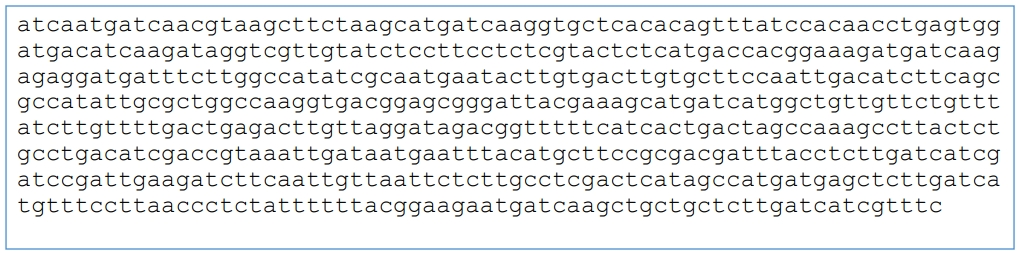
\includegraphics[width=0.75\textwidth]{images/vibrio_cholerae.jpeg}
\caption{Početni region replikacije bakterije \textit{Vibrio cholerae} \cite{online_lecture}}
\label{figg:vibrio}
\end{figure}

Konkretno, u tom regionu izdvajaju se sledeći obrasci:
\texttt{ATGATCAAG} i \texttt{CTTGATCAT} (Slika \ref{figg:vibrio_1}). Ova dva obrasca predstavljaju međusobne reverzne komplemente, što znači da nose istu biološku informaciju posmatrano na komplementarnim DNK lancima. 

\begin{figure}[h]
\centering
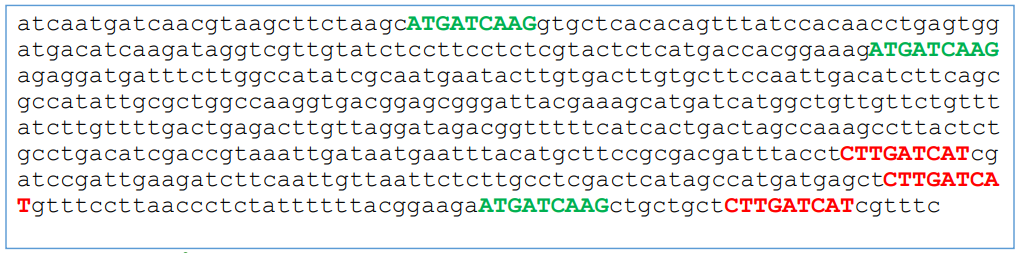
\includegraphics[width=0.75\textwidth]{images/vibrio_cholerae_2.jpeg}
\caption{Početni region replikacije   bakterije \textit{Vibrio cholerae} sa označenim 9-gramima koji se najčešće pojavljuju \cite{online_lecture}}
\label{figg:vibrio_1}
\end{figure}

Ono što ih čini posebno interesantnim jeste činjenica da se oba pojavljuju više puta i to u neposrednoj blizini, unutar istog kratkog regiona genoma. Važno je naglasiti da ovakva pojava nije verovatna u slučajnoj DNK sekvenci. Verovatnoća da se isti 9-mer pojavi više puta u kratkom segmentu genoma je veoma mala. Na primer, verovatnoća da se neki 9-mer pojavi tri ili više puta u slučajno generisanom DNK nizu dužine 500 iznosi približno $1/1300$. Zbog toga se ovakvi obrasci smatraju statistički značajnim, a upravo takvi grupisani motivi predstavljaju \textit{DnkA} boksove.

Važno je naglasiti da \textit{DnkA} boksovi nisu univerzalni i da je nukleotidni sastav \textit{DnkA} boksova specifičan za različite organizme. Na primer, analiza \textit{oriC} regiona bakterije \textit{Thermotoga petrophila}, prikazanog na Slici \ref{figg:thermotoga}, pokazuje da se obrasci \texttt{ATGATCAAG} i \texttt{CTTGATCAT}, koji su karakteristični za \textit{Vibrio cholerae}, u ovom genomu uopšte ne pojavljuju. Umesto toga, izdvajaju se drugačiji često zastupljeni 9-grami, kao što su \texttt{AACCTACCA}, \texttt{ACCTACCAC},  \texttt{CCTACCACC} i drugi slični motivi.

\begin{figure}[h]
\centering
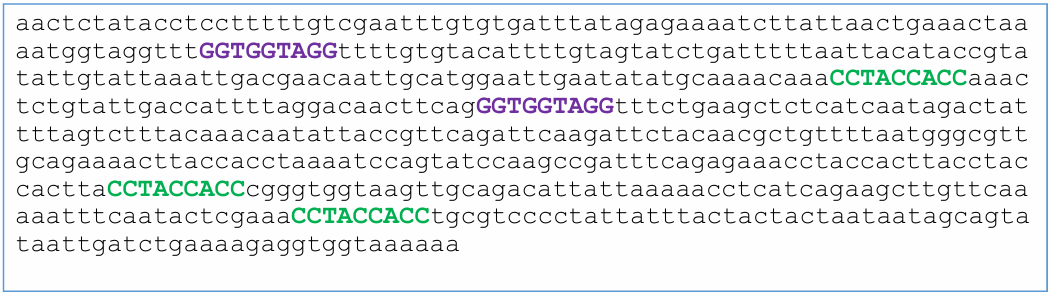
\includegraphics[width=0.75\textwidth]{images/thermotoga.png}
\caption{Početni region replikacije  bakterije \textit{Thermotoga petrophila} \cite{online_lecture}}
\label{figg:thermotoga}
\end{figure}

Da bismo formalizovali problem i započeli sa njegovim rešavanjem, ključna informacija je da se ovi obrasci pojavljuju lokalno grupisano. Zbog toga se uvodi problem pronalaženja grupa (eng. \textit{Clump Finding Problem}), čiji je cilj identifikacija $k$-grama koji se pojavljuju više puta unutar ograničenog regiona genoma.


\subsection{Algoritam}

Problem pronalaženja grupa formalno se definiše na sledeći način:

\begin{itemize}
    \item Ulaz: niska $Genome$ i celi brojevi $k$, $L$ i $t$
    \item Izlaz: svi različiti $k$-grami koji formiraju $(L,t)$-grupe u niski $Genome$
\end{itemize}

Kažemo da $k$-gram formira $(L,t)$-grupu ukoliko postoji podniska genoma dužine $L$ u kojoj se posmatrani $k$-gram pojavljuje najmanje $t$ puta.

Drugim rečima, traže se sve podsekvence dužine $k$ koje su lokalno učestale u makar jednom segmentu genoma dužine $L$.

\subsubsection{Naivni pristup}


Osnovna ideja algoritma zasniva se na korišćenju kliznog prozora dužine $L$ koji se pomera duž cele sekvence $Genome$. Za svaki položaj prozora posmatra se odgovarajući segment genoma, određuju se frekvencije svih $k$-grama u njemu, a zatim proverava da li se neki od njih pojavljuje najmanje $t$ puta.

Ako određeni $k$-gram zadovoljava ovaj uslov u makar jednom prozoru, smatra se da formira grupu i uključuje se u skup rezultata.


Najdirektniji pristup rešavanju ovog problema jeste da se za svaki prozor dužine $L$ iznova izračuna niz frekvencija svih $k$-grama. Nakon toga se prolazi kroz sve moguće indekse od $0$ do $4^k-1$ i proverava da li odgovarajući $k$-gram ima frekvenciju veću ili jednaku $t$.

Algoritam \ref{alg:clump_naive} prikazuje ovu osnovnu varijantu.

\begin{algorithm}[h]
\caption{Clump Finding}
\label{alg:clump_naive}
\SetAlgoLined
\DontPrintSemicolon
\SetKwFunction{FRec}{ClumpFinding}
\SetKwProg{Fn}{Funkcija}{}{}
\Fn{\FRec{Genome, k, L, t}}{
    $FrequentPatterns \gets$ prazan skup\;
    
    \For{$i \gets 0$ \KwTo $|Genome| - L$}{
        $Text \gets Genome[i..i+L-1]$\;
        $FrequencyArray \gets$ ComputingFrequencies$(Text, k)$\;

        \For{$index \gets 0$ \KwTo $4^k - 1$}{
            \If{$FrequencyArray[index] \ge t$}{
                $Pattern \gets$ NumberToPattern$(index, k)$\;
                dodaj $Pattern$ u $FrequentPatterns$\;
            }
        }
    }

    

    \Return{$FrequentPatterns$}
}
\end{algorithm}

\subsubsection{Primer}

Pretpostavimo da se duž genoma pomera prozor dužine $L = 500$ i da se u svakom takvom segmentu posmatraju 9-grami, odnosno da je $k = 9$. Ukoliko se određeni 9-gram pojavi najmanje $t = 3$ puta unutar nekog prozora, tada kažemo da on formira $(500,3)$-grupu.

Na primer, ukoliko se obrazac \texttt{ATGATCAAG} tri puta pojavi unutar jednog segmenta dužine 500 nukleotida, taj obrazac predstavlja kandidat za biološki značajnu sekvencu. Slično važi i za njegov reverzni komplement. Upravo ovakvi lokalno grupisani obrasci predstavljaju signal koji može ukazivati na prisustvo \textit{oriC} regiona.



\subsection{Vremenska složenost naivnog pristupa}

Vremenska složenost određuje se na osnovu broja prozora i broja operacija koje se izvršavaju unutar svakog od njih.

Broj prozora dužine $L$ u niski $Genome$ jednak je:
\[
|Genome| - L + 1
\]

Za svaki prozor najpre se računa niz frekvencija. Funkcija \textit{\textbf{ComputingFrequencies}} zahteva inicijalizaciju niza dimenzije $4^k$, što ima složenost $O(4^k)$, a zatim prolazak kroz prozor dužine $L$, pri čemu se za svaki od približno $L$ $k$-grama vrši transformacija pomoću funkcije \textit{\textbf{PatternToNumber}}. Kako ova transformacija obrađuje $k$ simbola, njen trošak je $O(k)$, pa ukupno računanje niza frekvencija zahteva:

\[
O(4^k + L \cdot k)
\]


 Kombinovanjem ovih koraka dobija se da je ukupna složenost jedne iteracije prozora:

\[
O(4^k + L \cdot k)
\]

Pošto se takva obrada vrši za svih $|Genome| - L + 1$ prozora, ukupna vremenska složenost naivnog algoritma iznosi:

\[
O((|Genome| - L + 1)\cdot(4^k + L\cdot k))
\]

Kako je uobičajeno da važi \(L \ll |Genome|\), broj prozora \((|Genome| - L + 1)\) može se aproksimirati sa \(|Genome|\), pa se vremenska složenost često zapisuje i kao

\[
O(|Genome| \cdot (4^k + L \cdot k)).
\]
Za velike genome ovaj pristup postaje veoma skup, jer se za svaki prozor iznova računa niz frekvencija bez korišćenja prethodnih rezultata. U tipičnom slučaju bakterijskih genoma, gde je $|Genome|$ veoma veliko, a $k$ i $L$ fiksirani, ova složenost je i dalje previsoka za efikasnu obradu.

\subsection{Optimizacija kliznog prozora}

Glavni nedostatak naivnog pristupa jeste to što se niz frekvencija pri svakom pomeranju prozora računa iz početka, iako se između dva uzastopna prozora menjaju frekvencije za veoma mali broj k-grama.

Kada se prozor pomeri za jednu poziciju udesno:
\begin{itemize}
    \item jedan $k$-gram izlazi iz prozora,
    \item jedan novi $k$-gram ulazi u prozor.
\end{itemize}

Sve ostale frekvencije ostaju nepromenjene. To znači da nije potrebno iznova računati ceo niz frekvencija, već je dovoljno ažurirati samo dve njegove vrednosti:
\begin{itemize}
    \item smanjiti frekvenciju $k$-grama koji izlazi iz prozora,
    \item povećati frekvenciju $k$-grama koji ulazi u prozor.
\end{itemize}

Na taj način dobija se efikasniji algoritam koji koristi isti princip kliznog prozora, ali izbegava redundantna izračunavanja.

\subsubsection{Optimizovani algoritam}

Algoritam \ref{alg:better_clump} prikazuje optimizovanu verziju pronalaženja grupa. U prvom koraku računa se niz frekvencija za početni prozor dužine $L$, a zatim se pri svakom pomeranju prozora ažuriraju samo vrednosti koje odgovaraju prvom i poslednjem $k$-gramu u novom položaju prozora.

\begin{algorithm}[h]
\caption{Better Clump Finding}
\label{alg:better_clump}
\SetAlgoLined
\DontPrintSemicolon
\SetKwFunction{FRec}{BetterClumpFinding}
\SetKwProg{Fn}{Funkcija}{}{}
\Fn{\FRec{Genome, k, t, L}}{
    $FrequentPatterns \gets$ prazan skup\;
    

    $Text \gets Genome[0..L-1]$\;
    $FrequencyArray \gets$ ComputingFrequencies$(Text, k)$\;

    \For{$i \gets 0$ \KwTo $4^k - 1$}{
        \If{$FrequencyArray[i] \ge t$}{

            $Pattern \gets$ NumberToPattern$(i, k)$\;
            dodaj $Pattern$ u $FrequentPatterns$\;
            
        }
    }

    \For{$i \gets 1$ \KwTo $|Genome| - L$}{
        $FirstPattern \gets Genome[i-1..i+k-2]$\;
        $indexFirst \gets$ PatternToNumber$(FirstPattern)$\;
        $FrequencyArray[indexFirst] \gets FrequencyArray[indexFirst] - 1$\;

        $LastPattern \gets Genome[i+L-k..i+L-1]$\;
        $indexLast \gets$ PatternToNumber$(LastPattern)$\;
        $FrequencyArray[indexLast] \gets FrequencyArray[indexLast] + 1$\;

        \If{$FrequencyArray[indexLast] \ge t$}{
            $Pattern \gets$ NumberToPattern$(indexLast, k)$\;
            dodaj $Pattern$ u $FrequentPatterns$\;
           
        }
    }

    

    \Return{$FrequentPatterns$}
}
\end{algorithm}

\subsection{Vremenska složenost optimizovanog pristupa}

Optimizovani algoritam najpre računa niz frekvencija za prvi prozor, što zahteva:

\[
O(4^k + L \cdot k)
\]

Nakon toga, za svaki naredni prozor vrše se dve transformacije pomoću funkcije \textit{\textbf{PatternToNumber}} i dve izmene u nizu frekvencija. Kako svaka transformacija zahteva $O(k)$ vremena, ukupni trošak jedne iteracije iznosi $O(k)$.

S obzirom na to da postoji $|Genome| - L$ pomeranja prozora, ukupni trošak ažuriranja frekvencija iznosi:

\[
O((|Genome| - L)\cdot k)
\]




Kombinovanjem svih koraka dobija se ukupna vremenska složenost optimizovanog algoritma:

\[
O(4^k \cdot k + L\cdot k + (|Genome| - L)\cdot k)
\]

Pošto važi

\[
L \cdot k + (|Genome| - L)\cdot k
=
|Genome| \cdot k,
\]

ukupna složenost može se zapisati kao

\[
O(4^k \cdot k + |Genome|\cdot k).
\]

Ovaj rezultat predstavlja značajno poboljšanje u odnosu na naivni pristup, jer se niz frekvencija više ne generiše iz početka za svaki prozor, čime se eliminiše multiplikativni faktor $L$.




\section{Asimetrija replikacije DNK i \textit{Skew} dijagram}

Proces replikacije DNK započinje u specifičnom regionu genoma poznatom kao \textit{oriC}, odakle se replikacija odvija u oba smera duž hromozoma, sve do regiona označenog kao \textit{terC} (eng.\textit{ termination of chromosomal replication}). Tokom ovog procesa formiraju se dve replikacione viljuške (eng. \textit{replication forks}), duž kojih se replikacija odvija u suprotnim smerovima.

DNK polimeraza sintetiše novi lanac na osnovu postojećeg, ali može da nadovezuje nukleotide isključivo u smeru $5' \rightarrow 3'$. Postavlja se pitanje na koji način se onda vrši sinteza novog lanca duž drugog lanca koji ima usmerenje $3' \rightarrow 5'$. Uslovljena orijentacija sinteze novog lanca dovodi do asimetrije u procesu replikacije i predstavlja osnovu za kasnije nastajanje razlika u raspodeli nukleotida duž genoma, o čemu će biti više reči u nastavku.



\subsection{Okazaki fragmenti i asimetrija replikacije}



Ograničenje da DNK polimeraza može da sintetiše novi lanac isključivo u smeru $5' \rightarrow 3'$ ima značajne posledice na proces replikacije. Iako se oba roditeljska lanca replikuju istovremeno, smer nastajanja duplikata nije isti.

Na osnovu smera replikacije, kružni bakterijski hromozom može se podeliti na dve polovine označene kao zaostajući (eng. \textit{forward half-strand}) i vodeći lanac (eng. \textit{reverse half-strand}). Na vodećem lancu DNK polimeraza može kontinuirano da prati otvaranje DNK molekula i sintetiše novi lanac bez prekida. Nasuprot tome, na zaostajućem lancu smer kretanja DNK polimeraze se razlikuje od orijentacije lanca, pa se sinteza ne može odvijati kontinualno.

Kao što je prikazano na Slici \ref{fig:half_strands}, hromozom se može podeliti na vodeći i na zaostajući lanac u odnosu na položaj početka replikacije (\textit{oriC}).

\begin{figure}[h]
\centering
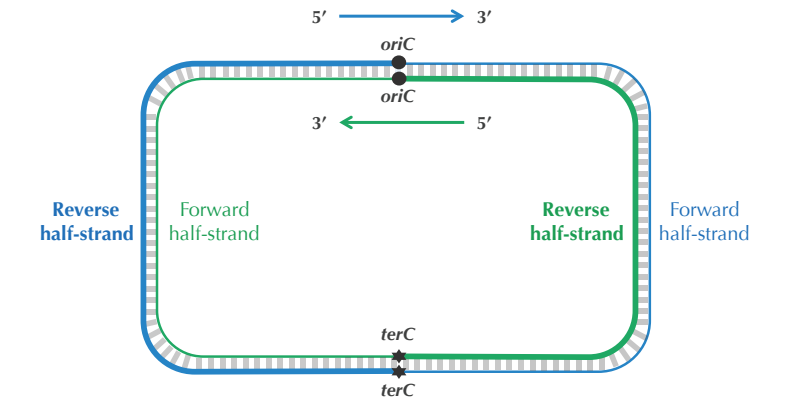
\includegraphics[width=0.75\textwidth]{images/forward_reverse_half_strands.png}
\caption{Vodeći i zaostajući lanac tokom procesa replikacije DNK \cite{online_book}.}
\label{fig:half_strands}
\end{figure}


Pošto DNK polimeraza ne može da sintetiše DNK u smeru $3' \rightarrow 5'$, na zaostajućem lancu neophodno je višestruko započinjanje sinteze. Svaki novi segment započinje formiranjem RNK prajmera, odnosno kratkog lanca RNK koji sintetiše enzim primaza i koji obezbeđuje početni $5'$ kraj sa koga DNK polimeraza može započeti sintezu. Ovi kratki DNK segmenti nazivaju se \textbf{Okazaki fragmenti}.

Kako se replikaciona viljuška pomera duž DNK molekula, nastaju novi Okazakijevi fragmenti, a DNK polimeraza periodično započinje sintezu novih fragmenata. Po završetku replikacije, RNK prajmeri se uklanjaju, njihovo mesto popunjavaju komplementarnim nukleotidima, a enzim DNK ligaza povezuje susedne fragmente u kontinuirani lanac. Zbog isprekidane sinteze, na zaostajućem lancu potreban je poseban RNK prajmer za svaki novonastali Okazaki fragment. Nasuprot tome, na vodećem lancu sinteza se odvija kontinualno, pa je dovoljan samo jedan RNK prajmer \cite{alberts2022}. 

Na Slici \ref{fig:replikacija1} prikazana je asimetrija replikacije DNK na vodećem i zaostajućem lancu, dok Slika \ref{fig:asimetrija} prikazuje ilustraciju koraka tokom replikacije.

\begin{figure}[h]
\centering
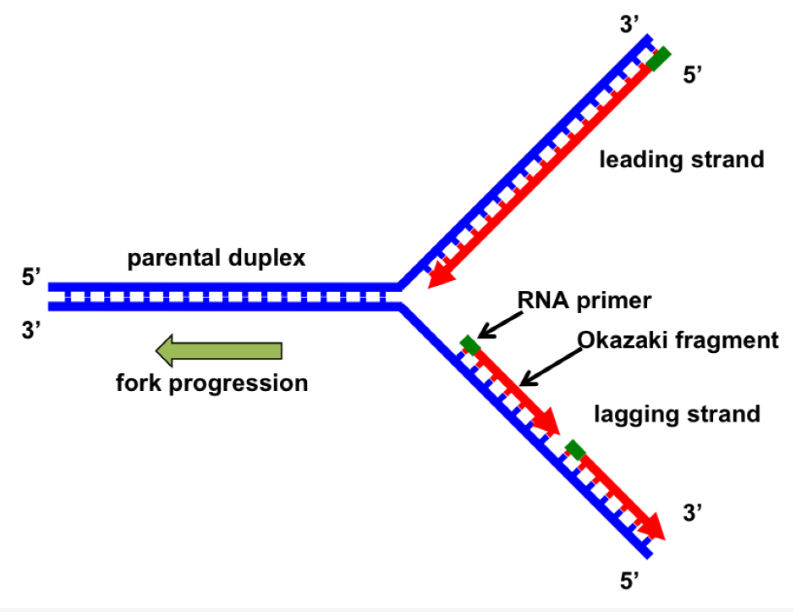
\includegraphics[width=0.75\textwidth]{images/asimetrija_replikacije.png}
\caption{Asimetrija replikacije na vodećem (leading) i zaostajućem (lagging) lancu \cite{leman2013}}
\label{fig:replikacija1}
\end{figure} 


\begin{figure}[h]
\centering
\resizebox{\textwidth}{!}{%
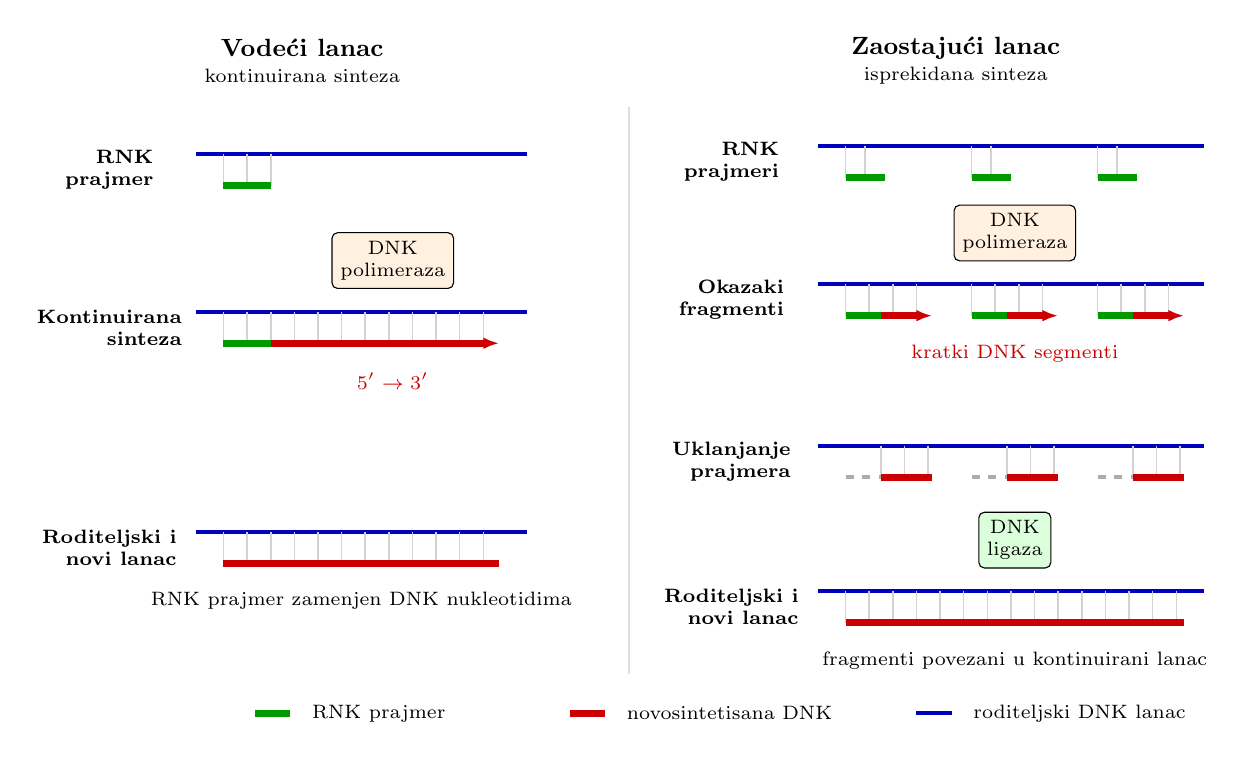
\begin{tikzpicture}[
    font=\scriptsize,
    >=Latex,
    parent/.style={blue!75!black, line width=1.4pt},
    pair/.style={gray!35, line width=0.55pt},
    dna/.style={red!80!black, line width=2.6pt},
    rna/.style={green!60!black, line width=2.6pt},
    gap/.style={gray!65, dashed, line width=1.2pt},
    enzyme/.style={
        draw,
        rounded corners=2pt,
        fill=orange!12,
        inner sep=3pt,
        align=center
    },
    ligase/.style={
        draw,
        rounded corners=2pt,
        fill=green!14,
        inner sep=3pt,
        align=center
    },
    title/.style={font=\bfseries\small, align=center},
    subtitle/.style={font=\scriptsize, align=center},
    label/.style={font=\scriptsize\bfseries, align=right},
    note/.style={font=\scriptsize, align=center}
]

% Titles
\node[title] at (3.7,0) {Vodeći lanac};
\node[subtitle] at (3.7,-0.35) {kontinuirana sinteza};

\node[title] at (12.0,0) {Zaostajući lanac};
\node[subtitle] at (12.0,-0.35) {isprekidana sinteza};

% Separator
\draw[gray!25] (7.85,-0.75) -- (7.85,-7.95);

% =====================================================
% REVERSE HALF-STRAND
% =====================================================

% Row 1
\node[label] at (1.25,-1.55) {RNK\\prajmer};
\draw[parent] (2.35,-1.35) -- (6.55,-1.35);
\foreach \x in {2.70,3.00,3.30}
    \draw[pair] (\x,-1.35) -- (\x,-1.75);
\draw[rna] (2.70,-1.75) -- (3.30,-1.75);

% Row 2
\node[label] at (1.25,-3.55) {Kontinuirana\\sinteza};
\draw[parent] (2.35,-3.35) -- (6.55,-3.35);
\foreach \x in {2.70,3.00,3.30,3.60,3.90,4.20,4.50,4.80,5.10,5.40,5.70,6.00}
    \draw[pair] (\x,-3.35) -- (\x,-3.75);
\draw[rna] (2.70,-3.75) -- (3.30,-3.75);
\draw[dna, -{Latex[length=2mm]}] (3.30,-3.75) -- (6.20,-3.75);
\node[enzyme] at (4.85,-2.70) {DNK\\polimeraza};
\node[note, red!80!black] at (4.85,-4.23) {$5' \rightarrow 3'$};

% Row 3
\node[label] at (1.25,-6.35) {Roditeljski i\\novi lanac};
\draw[parent] (2.35,-6.15) -- (6.55,-6.15);
\foreach \x in {2.70,3.00,3.30,3.60,3.90,4.20,4.50,4.80,5.10,5.40,5.70,6.00}
    \draw[pair] (\x,-6.15) -- (\x,-6.55);
\draw[dna] (2.70,-6.55) -- (6.20,-6.55);
\node[note] at (4.45,-7.02) {RNK prajmer zamenjen DNK nukleotidima};

% =====================================================
% FORWARD HALF-STRAND
% =====================================================

% Row 1
\node[label] at (9.15,-1.45) {RNK\\prajmeri};
\draw[parent] (10.25,-1.25) -- (15.15,-1.25);
\foreach \x in {10.60,10.85,12.20,12.45,13.80,14.05}
    \draw[pair] (\x,-1.25) -- (\x,-1.65);
\foreach \x in {10.60,12.20,13.80}
    \draw[rna] (\x,-1.65) -- ++(0.50,0);

% Row 2
\node[label] at (9.15,-3.20) {Okazaki\\fragmenti};
\draw[parent] (10.25,-3.00) -- (15.15,-3.00);
\foreach \x in {10.60,10.90,11.20,11.50,12.20,12.50,12.80,13.10,13.80,14.10,14.40,14.70}
    \draw[pair] (\x,-3.00) -- (\x,-3.40);

\draw[rna] (10.60,-3.40) -- (11.05,-3.40);
\draw[dna, -{Latex[length=2mm]}] (11.05,-3.40) -- (11.70,-3.40);

\draw[rna] (12.20,-3.40) -- (12.65,-3.40);
\draw[dna, -{Latex[length=2mm]}] (12.65,-3.40) -- (13.30,-3.40);

\draw[rna] (13.80,-3.40) -- (14.25,-3.40);
\draw[dna, -{Latex[length=2mm]}] (14.25,-3.40) -- (14.90,-3.40);

\node[enzyme] at (12.75,-2.35) {DNK\\polimeraza};
\node[note, red!80!black] at (12.75,-3.88) {kratki DNK segmenti};

% Row 3
\node[label] at (9.15,-5.25) {Uklanjanje\\prajmera};
\draw[parent] (10.25,-5.05) -- (15.15,-5.05);

\foreach \x in {11.05,11.35,11.65,12.65,12.95,13.25,14.25,14.55,14.85}
    \draw[pair] (\x,-5.05) -- (\x,-5.45);

\draw[gap] (10.60,-5.45) -- (11.05,-5.45);
\draw[dna] (11.05,-5.45) -- (11.70,-5.45);

\draw[gap] (12.20,-5.45) -- (12.65,-5.45);
\draw[dna] (12.65,-5.45) -- (13.30,-5.45);

\draw[gap] (13.80,-5.45) -- (14.25,-5.45);
\draw[dna] (14.25,-5.45) -- (14.90,-5.45);

% Row 4
\node[label] at (9.15,-7.10) {Roditeljski i\\novi lanac};
\draw[parent] (10.25,-6.90) -- (15.15,-6.90);
\foreach \x in {10.60,10.90,11.20,11.50,11.80,12.10,12.40,12.70,13.00,13.30,13.60,13.90,14.20,14.50,14.80}
    \draw[pair] (\x,-6.90) -- (\x,-7.30);
\draw[dna] (10.60,-7.30) -- (14.90,-7.30);
\node[ligase] at (12.75,-6.25) {DNK\\ligaza};
\node[note] at (12.75,-7.78) {fragmenti povezani u kontinuirani lanac};

% =====================================================
% LEGEND
% =====================================================

\begin{scope}[shift={(7.9,-8.45)}]
    \draw[rna] (-4.8,0) -- (-4.35,0);
    \node[note, anchor=west] at (-4.20,0) {RNK prajmer};

    \draw[dna] (-0.8,0) -- (-0.35,0);
    \node[note, anchor=west] at (-0.20,0) {novosintetisana DNK};

    \draw[parent] (3.6,0) -- (4.05,0);
    \node[note, anchor=west] at (4.20,0) {roditeljski DNK lanac};
\end{scope}

\end{tikzpicture}%
}
\caption{Uporedni prikaz asimetrije replikacije DNK na vodećem i zaostajućem lancu. Plavi segment označava roditeljski DNK lanac koji služi kao matrica, zeleni segmenti označavaju RNK prajmere, a crveni segmenti novosintetisanu DNK.}
\label{fig:asimetrija}
\end{figure}
Na Slici \ref{fig:okazaki_fragments} prikazan je proces formiranja Okazaki fragmenata i njihovo povezivanje u kontinuirani DNK lanac.

\begin{figure}[h]
\centering
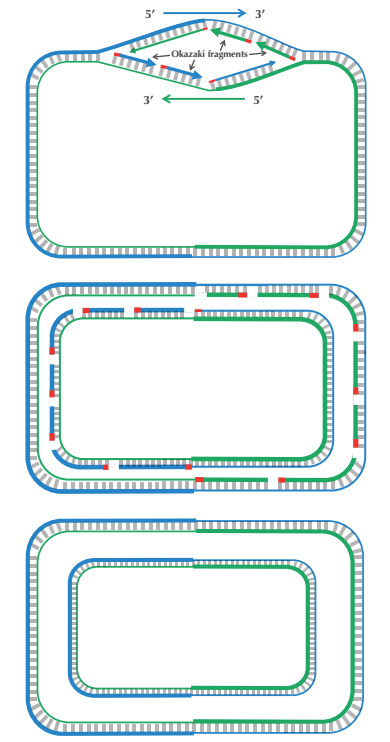
\includegraphics[width=0.5\textwidth]{images/okazaki_fragments.png}
\caption{Nastanak Okazaki fragmenata tokom replikacije i njihovo povezivanje u kontinuirani DNK lanac \cite{online_book}.}
\label{fig:okazaki_fragments}
\end{figure} 

Zbog stalnog započinjanja i prekidanja sinteze, zaostajući lanac provodi znatno više vremena u jednolančanom stanju od vodećeg lanca. 
Ova razlika između kontinuirane i isprekidane sinteze predstavlja osnovu za nastanak statističke asimetrije nukleotidnog sastava DNK u \textit{oriC} regionu.
 

Jednolančana DNK je hemijski nestabilnija i podložnija mutacijama. Posebno je značajan proces deaminacije, odnosno hemijski proces u kojem se iz molekula uklanja amino grupa. U ovom procesu dolazi do transformacije citozina u timin, što doprinosi promenama u nukleotidnom sastavu DNK. Ova mutacija se češće dešava na lancu koji duže ostaje jednolančan. Kao posledica toga, zaostajući lanac vremenom gubi citozin, što dovodi do neravnomerne raspodele nukleotida između dva dela genoma, posebno između baza guanin (G) i citozin (C).

 Ova asimetrija u raspodeli nukleotida predstavlja važan signal koji se može iskoristiti za identifikaciju početnog regiona replikacije. Naime, raspodela nukleotida razlikuje se između dve polovine hromozoma usled različitih uslova sinteze vodećeg i zaostajućeg lanca. U regionu \textit{oriC}, gde započinje replikacija, dolazi do promene ovog obrasca raspodele nukleotida, zbog čega se upravo taj region može identifikovati analizom nukleotidne asimetrije.

Da bi se ovaj fenomen formalizovao, uvodi se grafik koji grafički prikazuje razliku između pojavljivanja G i C duž genoma.


\subsection{Iskrivljeni dijagram}

\textit{GC-skew} predstavlja meru razlike između broja pojavljivanja baza guanin (G) i citozin (C) u prefiksu DNK sekvence.

Formalno, za poziciju $i$ definišemo meru:
\[
Skew(i) = \#G - \#C,
\]
gde $\#G$ i $\#C$ predstavljaju broj pojavljivanja baza G i C u prvih $i$ nukleotida sekvence.

Početna vrednost funkcije je:
\[
Skew(0) = 0
\]

\subsubsection{Konstrukcija iskrivljenog dijagrama}

Iskrivljeni dijagram (eng. \textit{Skew Diagram}) se konstruiše prolaskom kroz sekvencu i inkrementalnim ažuriranjem vrednosti funkcije.

Za svaku poziciju važi:
\begin{itemize}
\item ako je baza G → vrednost se povećava za 1
\item ako je baza C → vrednost se smanjuje za 1
\item ako je baza A ili T → vrednost ostaje nepromenjena
\end{itemize}

Na ovaj način dobija se niz vrednosti koji se može grafički prikazati, gde \textit{x}-osa predstavlja poziciju u genomu, a \textit{y}-osa vrednost funkcije $Skew(i)$.

Algoritam \ref{alg:skew} prikazuje pseudokod za izračunavanje \textit{GC-skew} vrednosti.

\begin{algorithm}[h]
\caption{Izračunavanje GC-skew}
\label{alg:skew}
\SetAlgoLined
\DontPrintSemicolon
\SetKwFunction{FRec}{GC-skew}
\SetKwProg{Fn}{Funkcija}{}{}
\Fn{\FRec{Genome}}{
$Skew[0] \gets 0$\;

\For{$i \gets 1$ \KwTo $|Genome|$}{
    $Skew[i] \gets Skew[i-1]$\;

    \If{$Genome[i] = G$}{
        $Skew[i] \gets Skew[i] + 1$\;
    }
    \ElseIf{$Genome[i] = C$}{
        $Skew[i] \gets Skew[i] - 1$\;
    }
}

\Return{$Skew$}
}
\end{algorithm}

\subsubsection{Interpretacija rezultata}

Vrednost funkcije $Skew(i)$ pokazuje karakterističan obrazac prilikom prolaska kroz genom. U jednom delu genoma vrednosti opadaju, dok u drugom počinju da rastu.

Tačka u kojoj funkcija dostiže minimum predstavlja mesto promene ovog trenda i u zapravo odgovara početnom regionu replikacije (\textit{oriC}). Intuitivno, minimum označava prelaz između dva dela genoma sa različitim statističkim osobinama, što je direktna posledica asimetrije procesa replikacije.

\subsubsection{Problem minimalnog \textit{skew}-a}

Na osnovu prethodne analize može se definisati problem pronalaženja minimalne vrednosti funkcije $Skew(i)$, koji predstavlja osnovu za algoritamsko određivanje lokacije \textit{oriC}. Cilj je pronaći sve pozicije u genomu na kojima funkcija dostiže svoju minimalnu vrednost, jer te pozicije predstavljaju kandidate za početni region replikacije (\textit{oriC}). Problem minimalnog \textit{skew}-a formalno se definiše na sledeći način:
\begin{itemize}
\item\textbf{Ulaz:} DNK sekvenca $Genome$.

\item\textbf{Izlaz:} sve pozicije $i$ za koje je vrednost $Skew(i)$ minimalna.
\end{itemize}

\subsubsection{Primer}

Na Slici \ref{fig:gc_skew_e} prikazan je \textit{GC-skew} dijagram za genom bakterije \textit{Escherichia coli}. 

Uočava se karakterističan obrazac u kome vrednost funkcije najpre raste, zatim opada i dostiže minimum, nakon čega ponovo počinje da raste. Ova promena trenda odražava prelaz između dva dela genoma sa različitim statističkim osobinama.

Minimum funkcije dostiže se približno na poziciji od oko 4 miliona nukleotida i predstavlja kandidat za lokaciju početnog regiona replikacije (\textit{oriC}). Razlog za to je što upravo na tom mestu dolazi do promene između zaostajućeg i vodećeg lanca, odnosno do promene u raspodeli baza G i C.

Takođe, u suprotnom delu genoma funkcija dostiže maksimum, što odgovara regionu približno nasuprot \textit{oriC} na kružnom hromozomu. Ova simetrična struktura dijagrama posledica je same prirode replikacije, koja se odvija u oba smera od početne tačke.

\begin{figure}[h]
\centering
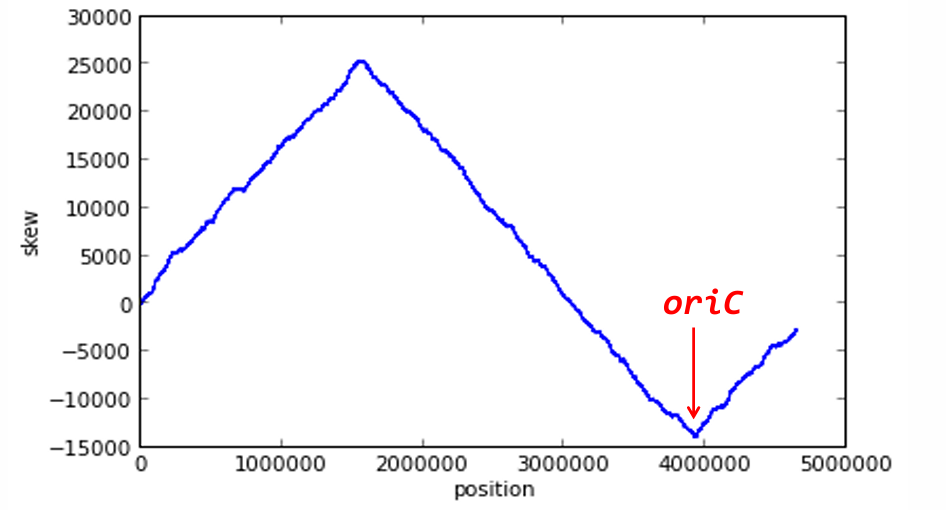
\includegraphics[width=0.7\textwidth]{images/gc_skew.png}
\caption{GC-skew dijagram za genom bakterije \textit{Escherichia coli} \cite{online_lecture}}
\label{fig:gc_skew_e}
\end{figure}

\subsection{Vremenska i prostorna složenost}

Algoritam za izračunavanje \textit{GC-skew} vrednosti zasniva se na jednom prolazu kroz DNK sekvencu. Za svaku poziciju u genomu vrši se ažuriranje vrednosti funkcije $Skew(i)$ na osnovu prethodne vrednosti, pri čemu se proverava samo trenutni nukleotid.

U svakom koraku izvršava se konstantan broj operacija, što znači da složenost po jednoj iteraciji iznosi $O(1)$.

Kako se ovaj postupak ponavlja za svih $|Genome|$ pozicija u sekvenci, ukupna vremenska složenost algoritma iznosi:
\[
O(|Genome|)
\]
Pored toga, potrebno je memorisati niz vrednosti dužine $|Genome|$, pa je prostorna složenost takođe:
\[
O(|Genome|).
\]

\subsection{Prednosti i ograničenja}

Jedna od glavnih prednosti ovog pristupa jeste njegova jednostavna implementacija, kao i činjenica da se zasniva na jednom prolazu kroz genom, što omogućava efikasno izračunavanje čak i za veoma duge sekvence. Dodatno, metoda ne zahteva unapred poznate obrasce u DNK, što je čini pogodnom za analizu genoma kod kojih relevantni motivi još uvek nisu identifikovani.

Sa druge strane, \textit{GC-skew} analiza ima i određena ograničenja. Pre svega, ona se oslanja na statističke osobine koje mogu varirati između različitih organizama, pa ne garantuje uvek precizno određivanje lokacije \textit{oriC} regiona. Takođe, uspešnost metode zavisi od izraženosti asimetrije u raspodeli nukleotida, koja u nekim genomima može biti slabo naglašena. Zbog toga se ovaj pristup, u praksi, najčešće koristi u kombinaciji sa algoritmima zasnovanim na analizi podniski, čime se postiže pouzdanija identifikacija biološki značajnih regiona.


\section{Približno poklapanje sekvenci i česte reči sa propustima}

U prethodnim poglavljima razmatrani su algoritmi zasnovani na tačnom poklapanju podniski u DNK sekvenci. Takav pristup podrazumeva da se funkcionalno značajni obrasci pojavljuju u potpuno identičnom obliku. Međutim, u realnim biološkim sistemima ova pretpostavka često nije zadovoljena zato što su DNK sekvence podložne mutacijama. Tada dolazi do zamene pojedinačnih nukleotida, pa se isti biološki motiv može pojaviti u više varijanti koje se razlikuju na manjem broju pozicija, ali i dalje zadržavaju svoju funkciju.


Zbog toga algoritmi zasnovani isključivo na tačnom poklapanju mogu propustiti značajne obrasce. Da bi se ovaj problem prevazišao, uvodi se model približnog poklapanja sekvenci, koji omogućava poređenje uz dozvoljeni broj odstupanja. Ovaj model predstavlja prirodno proširenje prethodnih pristupa i čini osnovu za rešavanje problema čestih reči sa propustima.

\subsection{Hamingovo rastojanje}

Osnovna mera razlike između sekvenci jednake dužine jeste Hamingovo rastojanje (eng. \textit{Hamming distance}). Za dve sekvence $p$ i $q$ dužine $k$, Hamingovo rastojanje definiše se kao broj pozicija na kojima se one razlikuju.

Ako su date sekvence
\[
p = p_1 p_2 \dots p_k
\quad \text{i} \quad
q = q_1 q_2 \dots q_k,
\]
onda se Hamingovo rastojanje može formalno zapisati kao:
\[
HammingDistance(p, q) = |\{ i \mid p_i \neq q_i \}|.
\] 

Na primeru sa Slike \ref{fig:hamming_primer}, sekvence \texttt{ATCGTAGC} i \texttt{ATGGTCGC} razlikuju se u dve pozicije, pa je njihovo Hamingovo rastojanje jednaka 2.

\begin{figure}[h]
\centering
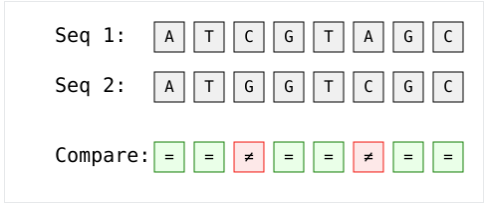
\includegraphics[width=0.65\textwidth]{images/hamming.png}
\caption{ Poređenje dve DNK sekvence sa naglašenim razlikama po pozicijama \cite{hamming_datacamp}}
\label{fig:hamming_primer}
\end{figure}
 
Ova mera predstavlja osnovni alat za procenu sličnosti između podniski. Što je Hamingovo rastojanje manje, to su dve sekvence međusobno sličnije.

\subsubsection{Algoritam za računanje Hamingovog rastojanja}

Najjednostavniji način računanja Hamingovog rastojanja zasniva se na poređenju odgovarajućih karaktera u dve sekvence iste dužine. Svaki put kada se simboli razlikuju, brojač se uvećava za 1. Algoritam \ref{alg:hamming_distance} prikazuje pseudokod ove funckije.

\begin{algorithm}[h]
\caption{Hamming Distance}
\label{alg:hamming_distance}
\SetAlgoLined
\DontPrintSemicolon
\SetKwFunction{FRec}{HammingDistance}
\SetKwProg{Fn}{Funkcija}{}{}
\Fn{\FRec{p, q}}{
$d \gets 0$\;

\For{$i \gets 1$ \KwTo $|p|$}{
    \If{$p_i \neq q_i$}{
        $d \gets d + 1$\;
    }
}

\Return{$d$}
}
\end{algorithm}

Ovaj algoritam prolazi kroz obe sekvence samo jednom i pri svakoj iteraciji proverava da li se simboli na istoj poziciji razlikuju. Zbog toga, njegova vremenska složenost je linearna u odnosu na dužinu sekvence.

\subsection{Približno poklapanje obrazaca}

Na osnovu Hamingovog rastojanja definiše se problem približnog poklapanja obrazaca (eng. \textit{Approximate Pattern Matching}). Za razliku od tačnog poklapanja, gde se zahteva potpuno podudaranje sekvenci, ovde se dozvoljava ograničen broj odstupanja.

Problem približnog poklapanja obrazaca formalno se definiše na sledeći način:

\begin{itemize}

\item\textbf{Ulaz:} niske $Text$ i $Pattern$, i ceo broj $d$ 

\item\textbf{Izlaz:} sve pozicije u $Text$ na kojima se $Pattern$ pojavljuje sa najviše $d$ odstupanja
\end{itemize}
Drugim rečima, traže se sve podniske dužine $|Pattern|$ čije je Hamingovo rastojanje od obrasca $Pattern$ manja ili jednaka $d$.



\subsubsection{Algoritam za približno poklapanje}

Najjednostavniji pristup rešavanju ovog problema zasniva se na kliznom prozoru. Prozor dužine $|Pattern|$ pomera se kroz sekvencu $Text$, a za svaku poziciju računa se Hamingovo rastojanje između obrasca i odgovarajuće podniske. Algoritam \ref{alg:approximate_pattern_matching} prikazuje pseudokod ove funcije.

\begin{algorithm}[h]
\caption{Approximate Pattern Matching}
\label{alg:approximate_pattern_matching}
\SetAlgoLined
\DontPrintSemicolon
\SetKwFunction{FRec}{ApproximatePatternMatching}
\SetKwProg{Fn}{Funkcija}{}{}
\Fn{\FRec{Text, Pattern, d}}{
$positions \gets$ prazan skup\;

\For{$i \gets 0$ \KwTo $|Text| - |Pattern|$}{
    $Pattern' \gets Text[i..i+|Pattern|-1]$\;

    \If{$HammingDistance(Pattern, Pattern') \le d$}{
        dodaj $i$ u $positions$\;
    }
}

\Return{$positions$}
}
\end{algorithm}

\subsubsection{Objašnjenje rada algoritma}

Algoritam sistematski razmatra sve podniske dužine $|Pattern|$ u tekstu. Za svaku od njih vrši se poređenje sa obrascem karakter po karakter, pri čemu se prebrojava broj pozicija na kojima se razlikuju.

Ukoliko broj razlika ne prelazi zadatu vrednost $d$, smatra se da na toj poziciji postoji približno poklapanje, pa se indeks te pozicije beleži u skup rezultata.

Važno je naglasiti da se i u ovom slučaju uzimaju u obzir preklapajuća pojavljivanja, jer se klizni prozor pomera za jednu poziciju u svakom koraku.

\
\subsubsection{Primer}

Posmatrajmo DNK sekvencu:
\[
\texttt{AACAAGCATAAACATTAAAGAG}
\]
i obrazac:
\[
\texttt{AAAAA},
\]
uz dozvoljeno $d = 2$.

Algoritam koristi klizni prozor dužine 5 i za svaku poziciju $i$ posmatra podnisku $Text[i..i+4]$, nakon čega računa Hamingovo rastojanje ($d_H$) u odnosu na obrazac.

Na primer:

\begin{itemize}
    \item Za $i = 0$: podniska je \texttt{AACAA}.  
    Poređenjem sa \texttt{AAAAA} dobijamo razliku na jednoj poziciji, pa je $d_H = 1$ i ova pozicija se prihvata.

    \item Za $i = 1$: podniska je \texttt{ACAAG}.  
    Razlikuje se u dve pozicije, pa je $d_H = 2$ i ova pozicija se prihvata.

    \item Za $i = 2$: podniska je \texttt{CAAGC}.  
    Razlikuje se u više od dve pozicije, pa se odbacuje.

    \item Za $i = 8$: podniska je \texttt{AAAAC}.  
    Razlikuje se u jednoj poziciji, pa je $d_H = 1$ i ova pozicija se prihvata.
\end{itemize}

Na ovaj način algoritam prolazi kroz celu sekvencu i vraća sve indekse na kojima se pojavljuje približno poklapanje, odnosno gde je Hamingovo rastojanje manje ili jednako $d$.

\subsection{Prebrojavanje približnih pojavljivanja}

Pored pronalaženja pozicija na kojima se obrazac pojavljuje sa odstupanjima, često je potrebno izračunati i ukupan broj takvih pojavljivanja. Zbog toga se uvodi funkcija:
\[
ApproximatePatternCount(Text, Pattern, d),
\]
koja vraća broj podniski u tekstu čije je Hamingovo rastojanje od obrasca $Pattern$ manje ili jednako $d$.



\begin{algorithm}[h]
\caption{Approximate Pattern Count}
\label{alg:approximate_pattern_count}
\SetAlgoLined
\DontPrintSemicolon
\SetKwFunction{FRec}{ApproximatePatternCount}
\SetKwProg{Fn}{Funkcija}{}{}
\Fn{\FRec{Text, Pattern, d}}{
$count \gets 0$\;

\For{$i \gets 0$ \KwTo $|Text| - |Pattern|$}{
    $Pattern' \gets Text[i..i+|Pattern|-1]$\;

    \If{$HammingDistance(Pattern, Pattern') \le d$}{
        $count \gets count + 1$\;
    }
}

\Return{$count$}
}
\end{algorithm}



Pseudokod je prikazan u Algoritmu \ref{alg:approximate_pattern_count} i veoma je sličan prethodnom, ali se umesto čuvanja svih pozicija računa samo brojač. Svaki put kada se pronađe podniska koja se razlikuje u najviše $d$ pozicija, brojač se povećava za 1.

Na kraju, algoritam vraća ukupan broj približnih pojavljivanja, odnosno vrednost funkcije $ApproximatePatternCount$.

\subsection{Vremenska složenost približnog poklapanja}

Algoritam za približno poklapanje prolazi kroz sve podniske dužine $|Pattern|$, kojih ima $|Text| - |Pattern| + 1$. Za svaku od njih računa se Hamingovo rastojanje, što zahteva $O(|Pattern|)$ operacija.

Zbog toga ukupna vremenska složenost iznosi:
\[
O(|Text| \cdot |Pattern|)
\]

Ova složenost je linearna u odnosu na dužinu teksta, ali zavisi i od dužine obrasca. Za kraće obrasce algoritam je efikasan, dok za duže sekvence ili veliki broj poređenja može postati zahtevniji.



\subsection{Problem čestih reči sa propustima}

Približno poklapanje i približno prebrojavanje pojavljivanja obrazaca predstavljaju osnovu za definisanje složenijeg problema. Sada cilj nije pronaći poklapanje sa datim obrascem, već pronaći najčešće obrasce kada su dozvoljena odstupanja.

Drugim rečima, ako za dati obrazac možemo da izračunamo koliko puta se pojavljuje u tekstu sa najviše $d$ razlika, tada možemo pokušati da pronađemo one obrasce koji maksimizuju ovu vrednost. Na taj način dolazimo do problema čestih reči sa propustima (eng. \textit{Frequent Words with Mismatches}).

Ovaj problem se može definisati na sledeći način:

\begin{itemize}
    \item \textbf{Ulaz:} niska $Text$, dužina $k$ i maksimalan broj dozvoljenih odstupanja $d$
    \item \textbf{Izlaz:} svi $k$-grami koji maksimizuju vrednost funkcije
    
    $ApproximatePatternCount(Text, Pattern, d)$
\end{itemize}

Za razliku od standardnog problema čestih reči, ovde frekvencija obrasca ne zavisi od broja tačnih poklapanja, već od broja približnih poklapanja. To znači da obrazac sa propustima  koji je najčešći ne mora nužno da se pojavljuje u tekstu u svom originalnom obliku. Upravo to čini ovaj problem složenijim i istovremeno biološki značajnijim.



\subsection{$d$-susedstvo obrasca}


Kod problema tačnih poklapanja, prilikom razmatranje kandidata za motiv (eng. \textit{pattern}), bilo je dovoljno posmatrati one $k$-grame koji se zaista pojavljuju u tekstu. Ovde to više nije slučaj. Razlog za to je što se k-gram koji ima najveći broj približnih pojavljivanja ne mora pojaviti u tekstu. Moguće je da se više podniski iz teksta razlikuje od nekog zajedničkog motiva u jednoj ili dve pozicije, i da upravo taj „centralni“ motiv ima najveću približnu frekvenciju, iako se s\^am nikada ne pojavljuje u svom originalnom obliku. Zbog toga je potrebno razmotriti ne samo postojeće podniske, već i njihove varijacije.


Za dati obrazac $Pattern$, njegovo $d$-susedstvo, označeno sa $Neighbors(Pattern, d)$, predstavlja skup svih sekvenci iste dužine koje se razlikuju od $Pattern$ u najviše $d$ pozicija.

Na primer, ako je dozvoljeno jedno odstupanje, tada susedstvo nekog obrasca sadrži sve sekvence koje se od njega razlikuju u najviše jednoj poziciji. Kako broj dozvoljenih odstupanja raste, susedstvo postaje sve veće.

Pojam susedstva je ključan zato što omogućava da se pretraga ograniči na skup kandidata koji su biološki smisleni, odnosno na sekvence koje su dovoljno bliske onima koje se zaista pojavljuju u tekstu.

\subsubsection{Generisanje $d$-susedstva}

Funkcija \texttt{Neighbors(Pattern, d)} može se implementirati rekurzivno. Osnovna ideja rekurzije zasniva se na tome da se prvo generišu "direktni" susedi sufiksa obrasca, odnosno oni na rastojanju 1, a zatim se u zavisnosti od njihovog Hamingovog rastojanja dodaje odgovarajući simbol na početak. Na ovaj način se korak po korak generišu sve sekvence koje zadovoljavaju uslov da se razlikuju od početnog obrasca u najviše $d$ pozicija. Pseudokod prikazan je u Algoritmu \ref{alg:neighbors}.

\begin{algorithm}[h]
\caption{Neighbors}
\label{alg:neighbors}
\SetAlgoLined
\DontPrintSemicolon
\SetKwFunction{FRec}{Neighbors}
\SetKwProg{Fn}{Funkcija}{}{}
\Fn{\FRec{Pattern, d}}{
\If{$d = 0$}{
    \Return{$\{Pattern\}$}\;
}

\If{$|Pattern| = 1$}{
    \Return{$\{A, C, G, T\}$}\;
}

$Neighborhood \gets$ prazan skup\;
$SuffixNeighbors \gets Neighbors(Suffix(Pattern), d)$\;

\ForEach{$Text \in SuffixNeighbors$}{
    \If{$HammingDistance(Suffix(Pattern), Text) < d$}{
        \ForEach{$x \in \{A, C, G, T\}$}{
            dodaj $x \cdot Text$ u $Neighborhood$\;
        }
    }
    \Else{
        dodaj $FirstSymbol(Pattern) \cdot Text$ u $Neighborhood$\;
    }
}

\Return{$Neighborhood$
}
}
\end{algorithm}

\subsubsection{Objašnjenje rada funkcije \textit{Neighbors}}

Ako je broj dozvoljenih odstupanja jednak nuli, jedini sused obrasca jeste sam obrazac. Ako je dužina obrasca jednaka 1, tada su svi simboli iz alfabeta mogući susedi.

U opštem slučaju najpre se rekurzivno generišu susedi maksimalnog sufiksa obrasca, koji se dobija uklanjanjem prvog karaktera. Zatim se za svaki takav sused proverava da li je njegovo Hamingovo rastojanje od originalnog sufiksa strogo manje od $d$. Ako jeste, na početak se može dodati bilo koji simbol, jer još uvek postoji prostor za dodatnu razliku. U suprotnom, mora se zadržati originalni prvi simbol, kako ukupan broj odstupanja ne bi prešao dozvoljenu vrednost.

\subsection{Algoritam za česte reči sa propustima}

Jedan od efikasnijih pristupa za rešavanje problema čestih reči sa propustima zasniva se na tome da se ne razmatra svih $4^k$ mogućih obrazaca, već samo oni koji pripadaju susedstvu nekog $k$-grama iz teksta.

U tu svrhu koriste se nizovi \textit{\texttt{Close}} i \textit{\texttt{FrequencyArray}}. Niz \textit{\texttt{Close}} sadrži identifikatore kandidata, dok \textit{\texttt{FrequencyArray}} čuva broj njihovih približnih pojavljivanja. Algoritam \ref{alg:frequent_words_with_mismatches} prikazuje pseudokod ove funkcije \textit{Frequent Words with Mismatches}.

\begin{algorithm}[h]
\caption{Frequent Words with Mismatches}
\label{alg:frequent_words_with_mismatches}
\SetAlgoLined
\DontPrintSemicolon
\SetKwFunction{FRec}{FrequentWordsWithMismatches}
\SetKwProg{Fn}{Funkcija}{}{}
\Fn{\FRec{Text, k, d}}{
$FrequentPatterns \gets$ prazan skup\;

\For{$i \gets 0$ \KwTo $4^k - 1$}{
    $Close[i] \gets 0$\;
    $FrequencyArray[i] \gets 0$\;
}

\For{$i \gets 0$ \KwTo $|Text| - k$}{
    $Neighborhood \gets Neighbors(Text[i..i+k-1], d)$\;

    \ForEach{$Pattern \in Neighborhood$}{
        $index \gets PatternToNumber(Pattern)$\;
        $Close[index] \gets 1$\;
    }
}

\For{$i \gets 0$ \KwTo $4^k - 1$}{
    \If{$Close[i] = 1$}{
        $Pattern \gets NumberToPattern(i, k)$\;
        $FrequencyArray[i] \gets ApproximatePatternCount(Text, Pattern, d)$\;
    }
}

$maxCount \gets$ maksimalna vrednost u $FrequencyArray$\;

\For{$i \gets 0$ \KwTo $4^k - 1$}{
    \If{$FrequencyArray[i] = maxCount$}{
        $Pattern \gets NumberToPattern(i, k)$\;
        dodaj $Pattern$ u $FrequentPatterns$\;
    }
}

\Return{$FrequentPatterns$}
}
\end{algorithm}

\subsubsection{Objašnjenje rada algoritma}

U prvom delu algoritma inicijalizuju se pomoćni nizovi. Nakon toga prolazi se kroz sve $k$-grame u tekstu, i za svaki od njih generiše se odgovarajuće $d$-susedstvo. Svaki obrazac iz tog susedstva označava se kao potencijalni kandidat.

U drugom delu algoritma prolazi se kroz sve moguće indekse. Ako je neki obrazac označen kao kandidat, za njega se računa vrednost funkcije \textit{\texttt{ApproximatePatternCount}}, odnosno broj približnih pojavljivanja u tekstu.

Na kraju se pronalazi maksimalna vrednost u nizu frekvencija i izdvajaju se svi obrasci koji postižu tu vrednost.

Važno je uočiti da se funkcija \textit{\texttt{ApproximatePatternCount}} ne poziva za svih $4^k$ mogućih k-grama, već samo za one koji pripadaju susedstvu nekog obrasca iz teksta. Time se postiže značajna ušteda u odnosu na iscrpnu pretragu.

\subsection{Uzimanje u obzir obrnutih komplementa}

U analizi DNK sekvenci nije dovoljno posmatrati samo jednu orijentaciju obrasca. Sekvenca i njen obrnuti komplement mogu imati istu biološku funkciju zato što se proteini mogu vezivati za motive prisutne na oba komplementarna lanca.

Zbog toga, ovaj problem se može dodatno proširiti tako da se za svaki obrazac posmatra i njegov obrnuti komplement. U tom slučaju frekvencija obrasca računa se kao zbir:
\[
ApproximatePatternCount(Text, Pattern, d)\] 
\[
+ 
\]
\[
ApproximatePatternCount(Text, ReverseComplement(Pattern), d)
\]

Na taj način se objedinuju obe moguće orijentacije iste informacije zapisane u DNK.

\subsubsection{Problem čestih reči sa propustima i obrnutim komplementima}

Kada se u obzir uzmu i obrnuti komplementi, problem se može definisati na sledeći način:

\begin{itemize}
    \item \textbf{Ulaz:} DNK sekvenca $Text$, dužina $k$ i maksimalan broj odstupanja $d$
    \item \textbf{Izlaz:} svi $k$-grami koji maksimizuju zbir približnih frekvencija svog oblika i svog obrnutog komplementa
\end{itemize}

Ova formulacija predstavlja realističniji model biološkog problema, jer uzima u obzir i prirodnu varijabilnost sekvenci i njihovu komplementarnost.


\subsection{Vremenska složenost}

Najveći izazov ovog pristupa jeste generisanje $d$-susedstva, što zavisi od njegove dimenzije. Za dati obrazac dužine $k$, broj suseda raste sa povećanjem broja dozvoljenih odstupanja $d$. Taj broj se može precizno izraziti formulom:

\[
\sum_{i=0}^{d} \binom{k}{i} \cdot 3^i,
\]
jer se za svaku od $i$ izmenjenih pozicija bira jedna od tri moguće alternativne baze.

Zbog toga, generisanje $d$-susedstva za sve $k$-grame u tekstu, kojih ima približno $|Text| - k + 1$, zahteva značajan broj operacija. Ukupan broj generisanih kandidata reda je veličine:

\[
O(|Text| \cdot 3^d \cdot k^d)
\]

Dodatni trošak nastaje u drugoj fazi algoritma, gde se za svakog kandidata računa vrednost funkcije \textit{\texttt{ApproximatePatternCount}}. Neka je broj različitih kandidata označen sa $C$. Kako funkcija \textit{\texttt{ApproximatePatternCount}} ima vremensku složenost $O(|Text| \cdot k)$, ukupni trošak ove faze iznosi:

\[
O(C \cdot |Text| \cdot k),
\]

gde važi:

\[
C \le \min(4^k,\ |Text| \cdot 3^d \cdot k^d).
\]

Pored toga, algoritam prolazi kroz nizove \textit{\texttt{Close}} i \textit{\texttt{FrequencyArray}} dužine $4^k$, pri čemu rekonstrukcija odgovarajućih obrazaca pomoću funkcije \textit{\texttt{NumberToPattern}} zahteva ukupno:

\[
O(4^k \cdot k).
\]

Kombinovanjem svih koraka dobija se ukupna vremenska složenost:

\[
O(|Text| \cdot 3^d \cdot k^d + C \cdot |Text| \cdot k + 4^k \cdot k).
\]

Ovaj rezultat pokazuje da algoritam ima visoku vremensku složenost, koja brzo raste sa povećanjem parametara $k$ i $d$. Iako pristup zasnovan na susedstvu značajno smanjuje broj kandidata u odnosu na potpuno iscrpnu pretragu, problem i dalje ostaje računarski zahtevan.




\subsection{Optimizovana implementacija za česte reči sa propustima}

Prethodno opisani pristup za rešavanje problema čestih reči sa propustima zasniva se na korišćenju nizova dimenzije $4^k$, što može predstavljati značajan nedostatak u pogledu memorijske efikasnosti. Kako vrednost $k$ raste, broj svih mogućih $k$-grama eksponencijalno se povećava, pa čuvanje informacija za svaki od njih postaje nepraktično.

Da bi se ovaj problem ublažio, može se primeniti optimizovani pristup zasnovan na korišćenju heš mape. Umesto da se unapred razmatraju svi mogući obrasci, u memoriji se čuvaju samo oni koji se pojavljuju u $d$-susedstvu nekog $k$-grama iz posmatranog teksta.

Ideja je da se prolazi kroz tekst i za svaki izdvojeni $k$-gram generiše njegovo $d$-susedstvo. Za svaki obrazac iz tog susedstva proverava se da li je već obrađen. Ako nije, izračunava se broj njegovih približnih pojavljivanja u tekstu i čuva u rečniku. Ključ u rečniku predstavlja obrazac, dok vrednost predstavlja broj njegovih približnih pojavljivanja.

Na ovaj način svaki kandidat se obrađuje najviše jednom, čime se izbegava nepotrebno ponavljanje izračunavanja, kao i čuvanje frekvencija za obrasce koji se uopšte ne pojavljuju kao relevantni kandidati.

\subsubsection{Algoritam}

Algoritam prolazi kroz tekst, generiše $d$-susedstvo za svaki $k$-gram i za svakog suseda računa približnu frekvenciju samo ako on već nije evidentiran u rečniku. Na kraju se iz rečnika izdvajaju svi obrasci koji imaju maksimalnu frekvenciju i oni predstavljaju najzastupljenije $k$-grame sa dozvoljenim odstupanjima \cite{matf_repo}. Pseudokod je prikazan u Algoritmu \ref{alg:fwwm_d}.

\begin{algorithm}[h]
\caption{Frequent Words with Mismatches (Dictionary)}
\label{alg:fwwm_d}
\SetAlgoLined
\DontPrintSemicolon
\SetKwFunction{FRec}{FrequentWordsWithMismatchesDictionary}
\SetKwProg{Fn}{Funkcija}{}{}
\Fn{\FRec{Text, k, d}}{
$FrequentPatterns \gets$ prazan skup\;
$FrequencyMap \gets$ prazna heš mapa\;

\For{$i \gets 0$ \KwTo $|Text| - k$}{
    $Pattern \gets Text[i..i+k-1]$\;
    $Neighborhood \gets Neighbors(Pattern, d)$\;

    \ForEach{$Neighbor \in Neighborhood$}{
        \If{$Neighbor$ nije ključ u $FrequencyMap$}{
            $FrequencyMap[Neighbor] \gets$ ApproximatePatternCount$(Text, Neighbor, d)$\;
        }
    }
}

$maxCount \gets$ maksimalna vrednost u $FrequencyMap$\;

\ForEach{$Pattern$ u $FrequencyMap$}{
    \If{$FrequencyMap[Pattern] = maxCount$}{
        dodaj $Pattern$ u $FrequentPatterns$\;
    }
}

\Return{$FrequentPatterns$}
}
\end{algorithm}



\subsubsection{Prednosti pristupa}

Glavna prednost ovog pristupa je smanjenje memorijske složenosti, jer se izbegava korišćenje nizova dimenzije $4^k$. Umesto toga, čuvaju se samo oni obrasci koji su zaista relevantni kandidati.

Pored toga, izbegava se i prolazak kroz sve moguće obrasce, pa se fokus stavlja isključivo na obrasce koji se javljaju u tekstu i njihove susede. Iako dominantni deo vremenske složenosti ostaje vezan za generisanje $d$-susedstva i računanje funkcije \textit{\texttt{ApproximatePatternCount}} za različite kandidate, ovaj pristup je u praksi memorijski efikasniji i jednostavniji za implementaciju.





\section{Ograničenja i otvoreni problemi}

U prethodnim poglavljima predstavljeni su algoritmi za analizu DNK sekvenci zasnovani na učestalosti podniski, njihovom lokalnom grupisanju i dozvoljenim odstupanjima. Iako ovi pristupi pružaju značajne uvide i omogućavaju identifikaciju potencijalno važnih obrazaca, njihova primena u realnim biološkim podacima otkriva niz ograničenja.

U nastavku ćemo razmotriti dodatne aspekte i otvorene probleme koji proizlaze iz ovih metoda.

\subsection{Ograničenja frekvencijskih pristupa}

Algoritmi poput \textit{Frequent Words} i \textit{Frequent Words with Mismatches} zasnivaju se na pretpostavci da su biološki značajni motivi ujedno i najčešće zastupljeni u sekvenci. Međutim, u praksi ova pretpostavka nije uvek validna.

U dugim DNK sekvencama određeni $k$-grami mogu se pojavljivati često isključivo kao posledica slučajnosti. Sa druge strane, funkcionalno važni motivi mogu biti prisutni u manjem broju kopija ili sa varijacijama, zbog čega ih frekvencijski pristupi ne detektuju pouzdano.

Uvođenjem dozvoljenih odstupanja povećava se fleksibilnost algoritma, ali istovremeno dolazi do značajnog povećanja broja kandidata, što može dovesti do pojave velikog broja lažno pozitivnih rezultata.

\subsubsection{Kombinatorna složenost i praktični izazovi}

Jedan od glavnih izazova jeste velika dimenzija prostora pretrage, budući da broj mogućih k-grama iznosi $4^k$. Ova kombinatorna eksplozija čini problem računarski zahtevnim, posebno za veće vrednosti parametara $k$ i $d$, prilikom generisanja $d$-susedstva. Iako optimizacije, poput korišćenja niza frekvencija i ograničavanja na relevantne kandidate, smanjuju broj operacija, algoritmi i dalje mogu biti spori za velike genomske sekvence.

\subsubsection{Statistički aspekti i verovatnoća obrazaca}

Važno pitanje koje se prirodno nameće jeste kako razlikovati obrasce koji su biološki značajni od onih koji su nastali slučajno. U tu svrhu neophodno je posmatrati verovatnoću pojavljivanja određenih podniski u sekvenci.

Ukoliko se neki obrazac pojavljuje češće nego što bi se očekivalo na osnovu slučajnog modela, može se smatrati potencijalno značajnim. Međutim, precizno modeliranje ovih verovatnoća predstavlja dodatni izazov i zahteva statističke metode koje prevazilaze osnovne algoritamske pristupe.

\subsection{Struktura DNK i dodatni biološki faktori}

Analiza DNK sekvenci ne zavisi samo od frekvencije podniski, već i od njihove biološke interpretacije. Na primer, značajnu ulogu imaju:

\begin{itemize}
    \item komplementarnost DNK lanaca i postojanje obrnutih komplementa,
    \item pravac (5' $\rightarrow$ 3') u kome se sekvence čitaju,
    \item preklapanje podniski, koje može uticati na statističku raspodelu obrazaca.
\end{itemize}

Ovi faktori dodatno komplikuju analizu i ukazuju na to da algoritamski rezultati moraju biti interpretirani u biološkom kontekstu.

\subsubsection{Otvoreni problemi u pronalaženju motiva}

Jedan od najvažnijih otvorenih problema jeste pronalaženje skrivenih motiva u DNK sekvencama. Za razliku od prethodnih problema, gde se analizirala jedna sekvenca, ovde se često posmatra više sekvenci i traži zajednički obrazac koji se u njima pojavljuje, ali ne nužno u identičnom obliku.

Ovaj problem je složen zato što:
\begin{itemize}
    \item motivi mogu sadržati mutacije,
    \item ne pojavljuju se na istim pozicijama,
    \item mogu biti maskirani šumom u podacima,
    \item nisu nužno najčešći obrasci u pojedinačnoj sekvenci.
\end{itemize}

Zbog toga standardni pristupi zasnovani na frekvenciji nisu dovoljni, već je potrebno razvijati naprednije algoritme koji kombinuju različite kriterijume.

\subsubsection{Primeri otvorenih problema}

U okviru savremene bioinformatike izdvajaju se i specifični problemi vezani za različite organizme:

\begin{itemize}
    \item identifikacija više početnih regiona replikacije u nekim bakterijama,
    \item pronalaženje \textit{oriC} regiona kod arheja, gde struktura genoma odstupa od bakterijske,
    \item analiza složenih eukariotskih genoma, kao što je kvasac, gde su regulatorni mehanizmi znatno kompleksniji.
\end{itemize}

Ovi problemi ukazuju na to da univerzalno rešenje ne postoji i da metode moraju biti prilagođene konkretnom biološkom sistemu.



Iako predstavljeni algoritmi čine osnovu za analizu DNK sekvenci, njihova ograničenja ukazuju na potrebu za daljim razvojem metoda u bioinformatici. Kombinacija algoritamskih tehnika, statističkih modela i biološkog znanja predstavlja ključ za uspešno rešavanje ovih problema. Zbog toga se savremena istraživanja fokusiraju na razvoj složenijih pristupa koji mogu pouzdanije identifikovati funkcionalno značajne motive u genomu.

% ------------------------------------------------------------------------------
\chapter{Elektronska lekcija}
% ------------------------------------------------------------------------------

U ovom poglavlju opisana je elektronska lekcija razvijena kao praktični deo rada. Lekcija je namenjena interaktivnom prikazu algoritama koji se koriste pri analizi DNK sekvenci i pronalaženju potencijalnog početnog regiona replikacije. Pored teorijskog objašnjenja pojmova, aplikacija omogućava korisniku da unese DNK sekvencu, pokrene odgovarajuće algoritme i prati njihove rezultate kroz vizuelni prikaz.

Elektronska lekcija se sastoji iz dve komponente: klijentske i serverske. Klijentska komponenta predstavlja korisnički interfejs aplikacije i implementirana je pomoću \textbf{\textit{Next.js}} \cite{nextjs} veb okvira, uz korišćenje biblioteka \textbf{\textit{React}} \cite{react} i \textbf{\textit{Node.js}} \cite{node}. Serverska komponenta implementirana je u programskom jeziku \textbf{\textit{Python}} \cite{python}, uz korišćenje \textbf{\textit{FastAPI}}\cite{fastapi} okvira. Izvorni kod aplikacije nalazi se u javnom \emph{\textit{GitHub}} \cite{github} repozitorijumu na adresi:
\begin{verbatim}
https://github.com/dunjaci/master-rad
\end{verbatim}

Aplikacija je javno dostupna preko sledeće adrese:
\begin{verbatim}
https://master-rad-seven.vercel.app
\end{verbatim}

Serverska komponenta dostupna je preko adrese:
\begin{verbatim}
https://master-rad-rynl.onrender.com/docs
\end{verbatim}


\section{Arhitektura aplikacije}

Aplikacija je organizovana kao sistem sa odvojenom klijentskom i serverskom komponentom. Klijentska komponenta je zadužena za prikaz stranica, unos podataka, navigaciju kroz lekciju i vizuelizaciju rezultata. Serverska komponenta obrađuje zahteve koje šalje klijentska aplikacija i izvršava algoritamsku logiku.

Ovakva organizacija omogućava jasnu podelu odgovornosti. Korisnički interfejs se razvija nezavisno od serverskog dela, dok se algoritmi i obrada podataka centralizuju u serverskoj komponenti. Na taj način se izbegava dupliranje algoritamske logike u klijentskoj aplikaciji, a rezultati koji se prikazuju korisniku dobijaju se preko definisanih API ruta.

Komunikacija između klijentske i serverske komponente ostvaruje se slanjem HTTP zahteva. Na primer, kada korisnik unese DNK sekvencu i izabere određene parametre, klijentska aplikacija šalje zahtev serverskoj komponenti, koja izvršava odgovarajući algoritam i vraća rezultat u JSON formatu.


\section{Korišćene tehnologije}

Klijentski deo aplikacije implementiran je korišćenjem \textbf{\textit{Next.js}} okvira.\textit{ Next.js} omogućava izradu \textit{React} aplikacija sa organizovanom strukturom stranica, jednostavnim rutiranjem i podrškom za produkcioni \textit{build}. Za stilizovanje korisničkog interfejsa korišćen je \textbf{\textit{Tailwind CSS}} \cite{tailwind}, što omogućava jednostavno kreiranje responzivnih i preglednih veb stranica.

Serverski deo aplikacije implementiran je pomoću \textbf{\textit{FastAPI}} okvira. \textit{FastAPI} je pogodan za izradu \textit{REST API-ja} jer omogućava jednostavno definisanje ruta, validaciju ulaznih podataka i automatski generisanu dokumentaciju programskog interfejsa. U ovoj aplikaciji serverska komponenta sadrži implementacije algoritama i vraća rezultate klijentskoj komponenti.

Za kontrolu verzija i čuvanje izvornog koda korišćen je \textbf{\textit{Git}} sistem, dok je repozitorijum postavljen na \textbf{\textit{GitHub}} platformu. Za javno postavljanje aplikacije korišćene su platforme \textbf{\textit{Render}} \cite{render} i \textbf{\textit{Vercel}} \cite{vercel}. Serverska komponenta postavljena je na \textit{Render}, dok je klijentska komponenta postavljena na \textit{Vercel}.


\section{Pokretanje aplikacije u lokalnom okruženju}

Aplikacija se može pokrenuti lokalno pokretanjem serverske i klijentske komponente u odvojenim terminalima. Serverska komponenta se nalazi u direktorijumu \texttt{\textit{backend}}, dok se klijentska komponenta nalazi u direktorijumu \texttt{\textit{frontend}}.

\subsection{Pokretanje serverske komponente}

Za pokretanje serverske komponente potrebno je pozicionirati se u direktorijum \texttt{\textit{backend}}. Nakon toga se instaliraju potrebne biblioteke iz datoteke \texttt{requirements.txt}. Serverska aplikacija se pokreće pomoću alata \texttt{\textit{uvicorn}}.

\begin{verbatim}
cd backend
pip install -r requirements.txt
uvicorn main:app --reload --port 8000
\end{verbatim}

Nakon pokretanja, serverska komponenta dostupna je na adresi:
\begin{verbatim}
http://localhost:8000
\end{verbatim}

Ispravnost rada serverske komponente može se proveriti otvaranjem sledeće adrese:
\begin{verbatim}
http://localhost:8000/api/health
\end{verbatim}

Ukoliko je server uspešno pokrenut, dobija se odgovor:
\begin{verbatim}
{"status":"ok"}
\end{verbatim}

\subsection{Pokretanje klijentske komponente}

Za pokretanje klijentske komponente potrebno je pozicionirati se u direktorijum \texttt{\textit{frontend}}. Zatim se instaliraju potrebni paketi i pokreće razvojni server.

\begin{verbatim}
cd frontend
npm install
npm run dev
\end{verbatim}

Nakon pokretanja, klijentskoj aplikaciji se može pristupiti preko adrese:
\begin{verbatim}
http://localhost:3000
\end{verbatim}

U lokalnom okruženju klijentska aplikacija podrazumevano šalje zahteve na adresu \texttt{http://localhost:8000}. Na taj način se lokalno pokrenuti frontend povezuje sa lokalno pokrenutim backend serverom.


\section{Postavljanje aplikacije na javno dostupne servise}

Da bi elektronska lekcija bila dostupna korisnicima preko javnog linka, aplikacija je postavljena na dve platforme. Serverska komponenta postavljena je na \textit{Render}, dok je klijentska komponenta postavljena na \textit{Vercel}. Ovakav pristup odgovara arhitekturi projekta jer su klijentski i serverski deo odvojeni.

\subsection{Postavljanje serverske komponente na \textit{Render}}

Serverska komponenta postavljena je na platformu \textit{Render} kao \emph{\textit{Web Service}}.\textit{ Render} je povezan sa \textit{GitHub} repozitorijumom, čime je omogućeno da se nova verzija serverske komponente automatski postavi nakon izmena u repozitorijumu.

\begin{figure}[h]
\centering
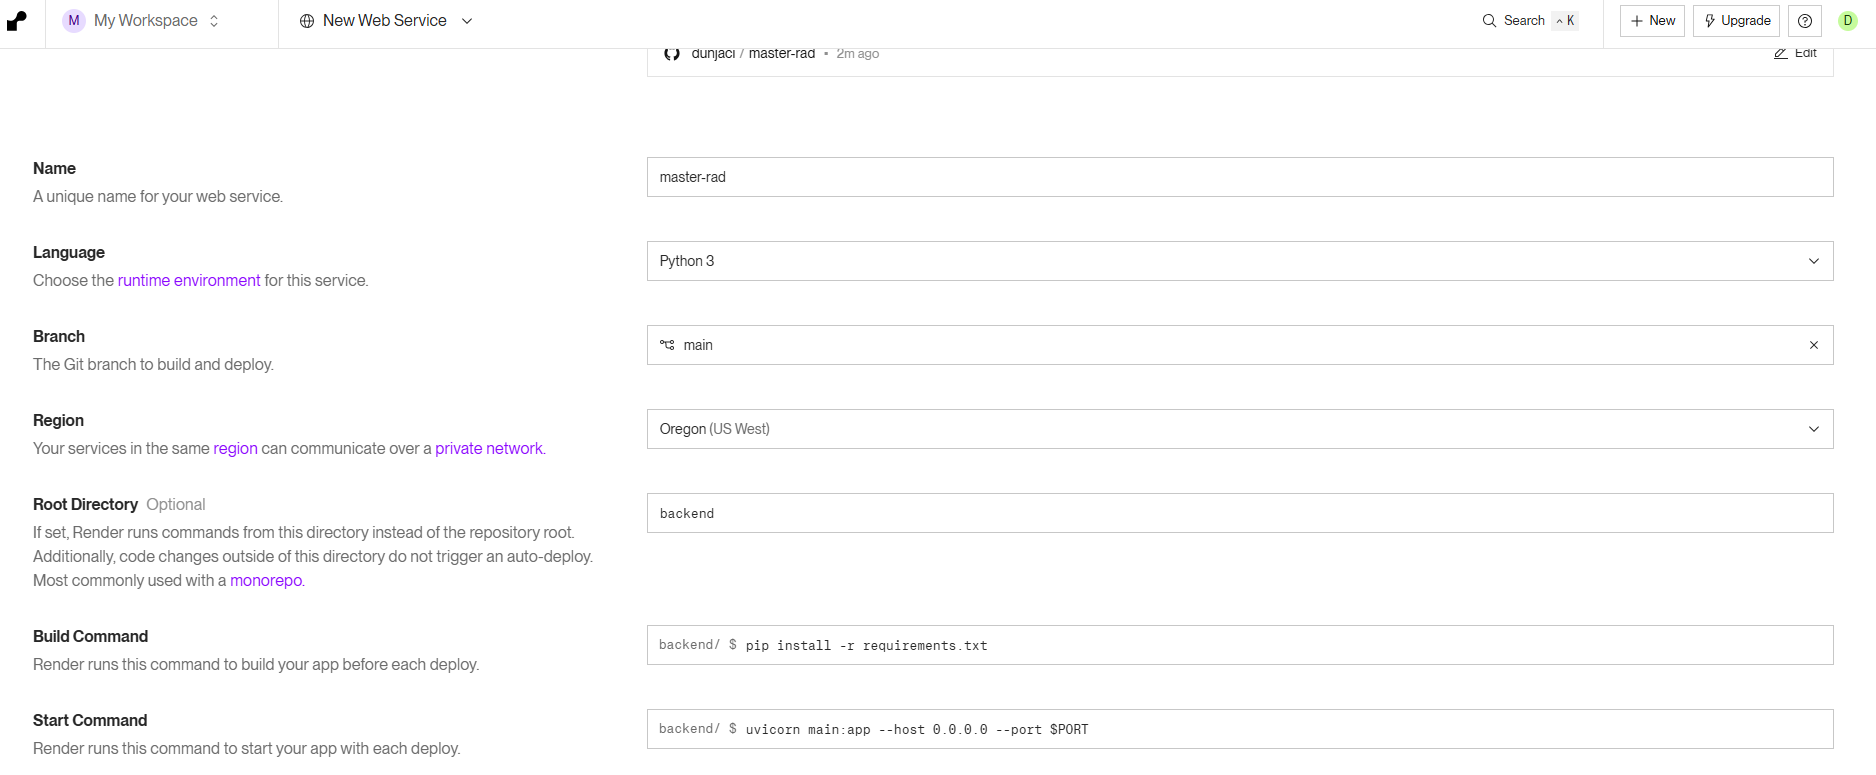
\includegraphics[width=1\textwidth]{images/depoloy_render.png}
\caption{Podešavanja za postavljanje (eng. \textit{deploy}) serverske komponente na Render platformu}
\label{fig:render_deploy}
\end{figure}


Kao što je prikazano na Slici \ref{fig:render_deploy}, prilikom kreiranja servisa podešeni su sledeći parametri:

\begin{verbatim}
Root Directory: backend
Runtime: Python
Build Command: pip install -r requirements.txt
Start Command: uvicorn main:app --host 0.0.0.0 --port $PORT
\end{verbatim}

Parametar \texttt{Root Directory} označava da se serverska komponenta nalazi u direktorijumu \texttt{backend}. Komanda za pripremu (eng. \textit{build command}) instalira sve zavisnosti navedene u datoteci \texttt{requirements.txt}, dok komanda za pokretanje startuje \textit{FastAPI} aplikaciju.

Nakon uspešnog postavljanja, \textit{Render} generiše javni URL serverske komponente:
\begin{verbatim}
https://master-rad-rynl.onrender.com
\end{verbatim}

\subsection{Postavljanje klijentske komponente na \textit{Vercel}}

Klijentska komponenta postavljena je na platformu \textit{Vercel}. \textit{Vercel} je posebno pogodan za \textit{Next.js} aplikacije jer automatski prepoznaje strukturu projekta i izvršava proces izgradnje aplikacije.


Slike \ref{fig::vercel_deploy} i \ref{figg:vercel_deploy_2} prikazuju podešavanja parametara prilikom kreiranja \textit{Vercel} projekta:

\begin{verbatim}
Root Directory: frontend
Framework Preset: Next.js
Build Command: npm run build
Install Command: npm install

\end{verbatim}
\begin{figure}[h]
\centering
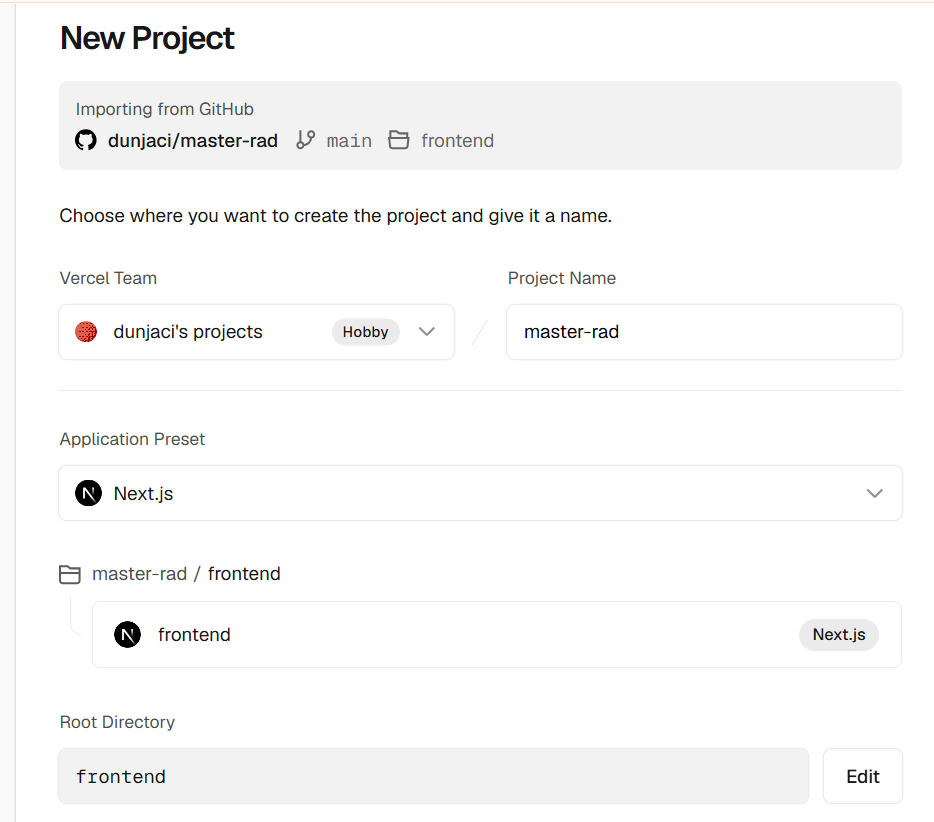
\includegraphics[width=0.75\textwidth]{images/vercel_deploy_1.png}
\caption{Podešavanja za postavljanje (eng. \textit{deploy}) klijentske komponente na Vercel platformu}
\label{fig::vercel_deploy}
\end{figure}

\begin{figure}[h]
\centering
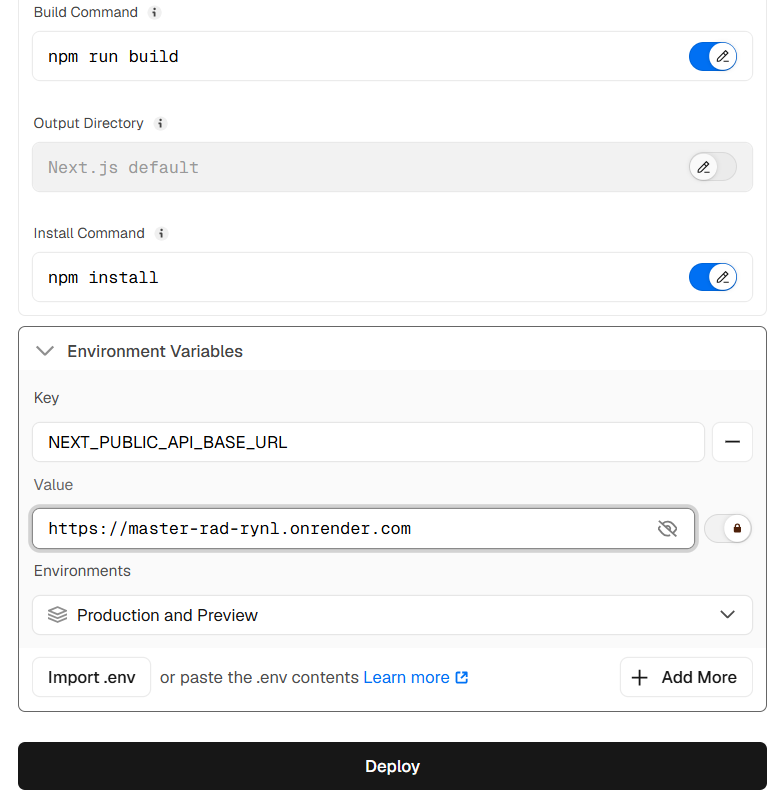
\includegraphics[width=0.75\textwidth]{images/vercel_deploy_2.png}
\caption{Podešavanja za deploy klijentske komponente na Vercel platformu}
\label{figg:vercel_deploy_2}
\end{figure}

\newpage
Pošto se klijentska aplikacija nalazi u direktorijumu \texttt{frontend}, taj direktorijum je označen kao korenski direktorijum projekta. Nakon uspešnog postavljanja, \textit{Vercel} generiše javnu adresu aplikacije:
\begin{verbatim}
https://master-rad-seven.vercel.app
\end{verbatim}

\subsection{Povezivanje klijentske i serverske komponente}

Povezivanje klijentske i serverske komponente ostvareno je pomoću promenljivih okruženja. Klijentska aplikacija koristi promenljivu \texttt{NEXT\_PUBLIC\_API\_BASE\_URL}, koja sadrži adresu serverske komponente:

\begin{verbatim}
NEXT_PUBLIC_API_BASE_URL=https://master-rad-rynl.onrender.com
\end{verbatim}

Na osnovu ove promenljive, klijentska aplikacija zna na koju adresu treba da šalje API zahteve. U lokalnom okruženju, ukoliko promenljiva nije definisana, koristi se podrazumevana adresa \texttt{http://localhost:8000}.

Sa druge strane, kao što je prikazano na Slici \ref{fig::render_add}, serverska komponenta koristi promenljivu \texttt{FRONTEND\_URL}, kojom se definiše sa kog domena je dozvoljeno slanje zahteva ka backend serveru:

\begin{verbatim}
FRONTEND_URL=https://master-rad-seven.vercel.app
\end{verbatim}

Ova promenljiva koristi se za podešavanje \textit{CORS} politike. Time se omogućava da produkciona verzija klijentske aplikacije komunicira sa serverskom komponentom, dok lokalna verzija i dalje može da koristi \texttt{http://localhost:3000}.

\begin{figure}[h]
\centering
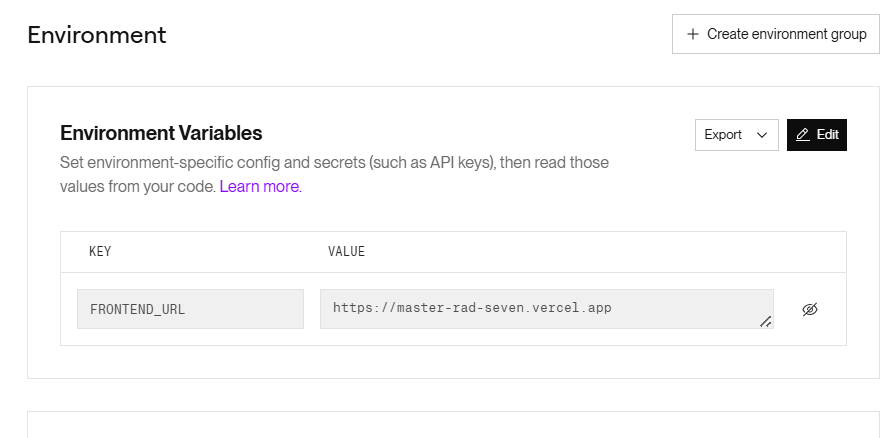
\includegraphics[width=0.75\textwidth]{images/render_add.png}
\caption{Podešavanja za povezivanje klijentske i serverske komponente}
\label{fig::render_add}
\end{figure}

Nakon povezivanja komponenti, tok komunikacije može se predstaviti na sledeći način:

\begin{verbatim}
Vercel frontend -> Render backend API -> rezultat se vraća korisniku
\end{verbatim}


\section{Funkcionalnosti elektronske lekcije}

Elektronska lekcija se sastoji iz više stranica koje zajedno prikazuju teorijski uvod, algoritme i literaturu. Na vrhu aplikacije nalazi se navigacioni meni preko kog korisnik može da pristupi svim delovima lekcije. Navigacija sadrži stranice: Uvod, Teorijske osnove, Česte reči, Pronalaženje grupa, \textit{GC-skew} dijagram, Propusti i Literatura. U navigaciji se nalazi i link ka GitHub repozitorijumu.

\subsection{Početna stranica}

Početna stranica predstavlja ulaznu tačku aplikacije (Slika \ref{fig:pocetna_stranica}). Na njoj je prikazan naslov lekcije i kratak pregled dostupnih celina. Korisnik sa ove stranice može da pređe na teorijske osnove, prikaze algoritama ili literaturu.

\begin{figure}[H]
\centering

\includegraphics[width=0.75\textwidth]{images/uvod.png}
\caption{Početna stranica elektronske lekcije}
\label{fig:pocetna_stranica}
\end{figure}

\subsection{Teorijske osnove}

Stranica Teorijske osnove, prikazana na Slici \ref{fig:teorijske_osnove}, uvodi biološke pojmove potrebne za razumevanje algoritama. Objašnjena je struktura DNK molekula, proces replikacije, početni region replikacije, DnkA boksovi i pojam obrnutog komplementa. Klikom na sekciju prikazuju se interaktivne kartice sa detaljnim objašnjenjima  pojmova. Ovaj deo lekcije povezuje biološku motivaciju sa algoritamskim problemima koji se kasnije obrađuju.

\begin{figure}[H]
\centering
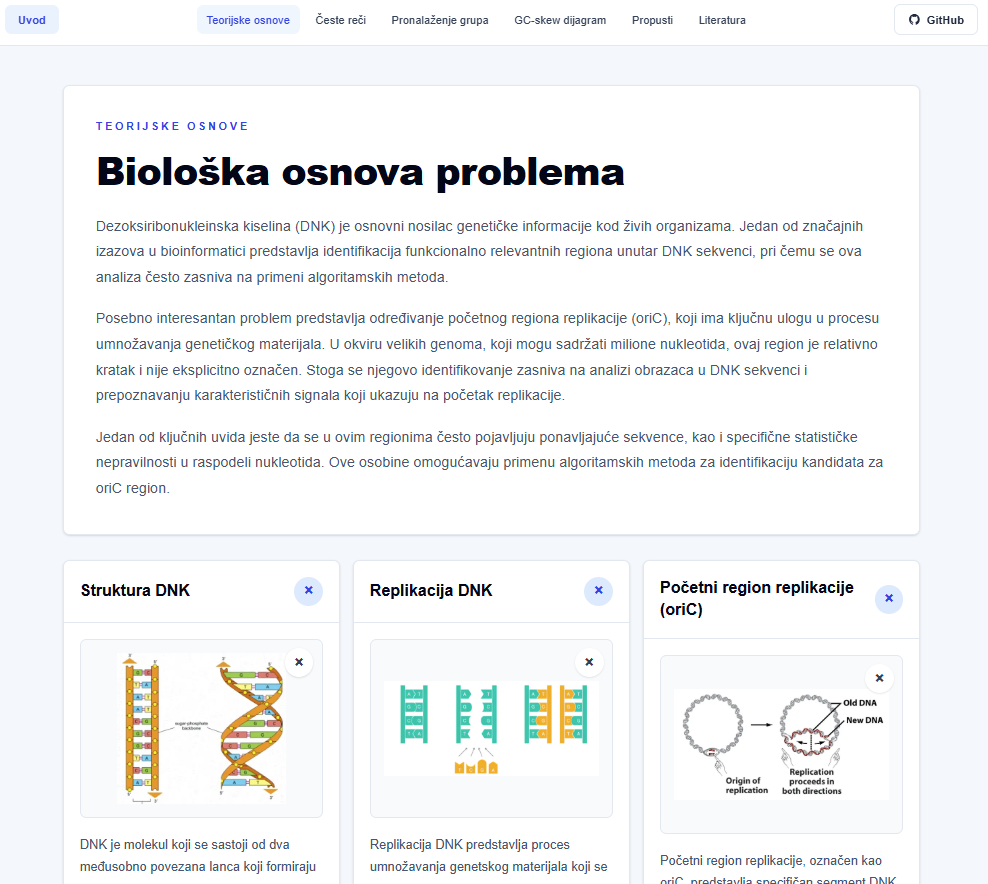
\includegraphics[width=0.75\textwidth]{images/teorijske_osnove.png}
\caption{Stranica sa teorijskim osnovama}
\label{fig:teorijske_osnove}
\end{figure}

\subsection{Česte reči}

Stranica Česte reči prikazuje algoritamski problem pronalaženja najčešćih k-grama u zadatoj DNK sekvenci. Korisnik može da unese sekvencu i vrednost parametra \texttt{k}. Aplikacija zatim prikazuje rezultat i omogućava praćenje rada različitih pristupa.

Na ovoj stranici predstavljeni su naivni algoritam, optimizacija nizom frekvencija, optimizacija heš mapom i pristup sortiranjem. Za svaki pristup prikazana je vremenska složenost, objašnjenje i programski kod u jeziku \textit{Python}. Vizuelni prikaz omogućava korisniku da prati trenutni k-gram, njegovu poziciju i način na koji algoritam obrađuje ulaznu sekvencu (Slika \ref{fig:ceste_reci}).

\begin{figure}[H]
\centering
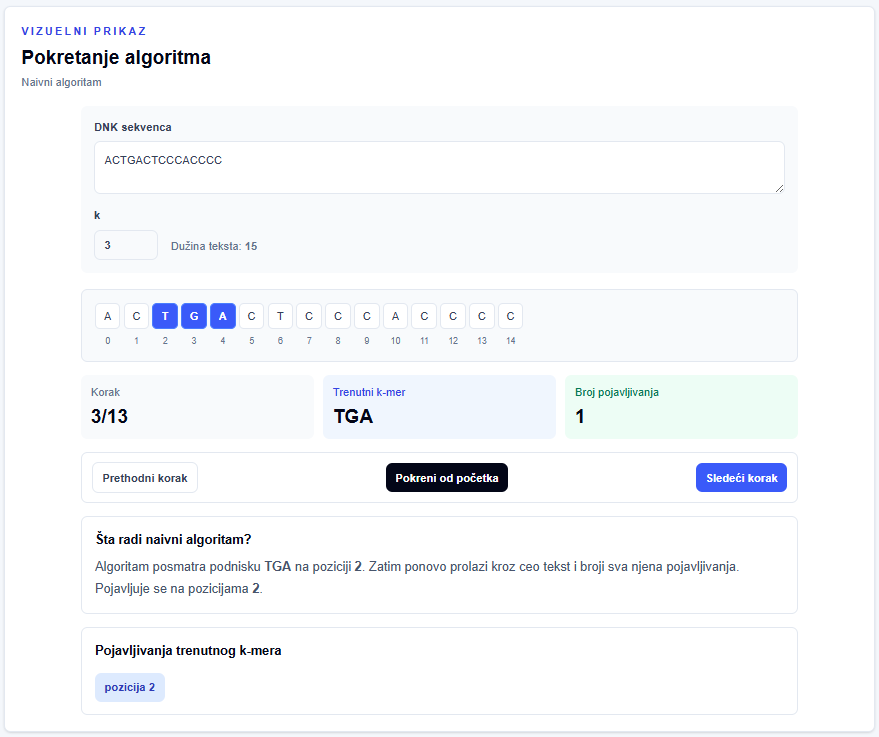
\includegraphics[width=0.75\textwidth]{images/ceste_reci.png}
\caption{Vizuelizacija naivnog algoritma za problem čestih reči}
\label{fig:ceste_reci}
\end{figure}

\subsection{Pronalaženje grupa}

Stranica Pronalaženje grupa prikazuje traženje k-grama koji formiraju \((L,t)\)-grupe. K-gram formira grupu ukoliko postoji segment genoma dužine \(L\) u kojem se taj k-gram pojavljuje najmanje \(t\) puta.

Korisnik unosi DNK sekvencu i parametre \texttt{k}, \texttt{L} i \texttt{t}. Aplikacija prikazuje prozore dužine \(L\), frekvencije k-grama u trenutnom prozoru i k-grame koji zadovoljavaju zadati prag. Pored osnovnog pristupa, prikazana je i optimizacija pomoću kliznog prozora, gde se pri svakom pomeranju prozora ažuriraju samo vrednosti za k-grame na granicama posmatranog segmenta (odnosno vrednosti za k-gram koji postaje obuhvaćen prozorom / prestaje da bude obuhvaćen prozorom). Vizuelizacija ovog pristupa prikazana je na Slici \ref{fig:pronalazenje_grupa}.

\begin{figure}[H]
\centering
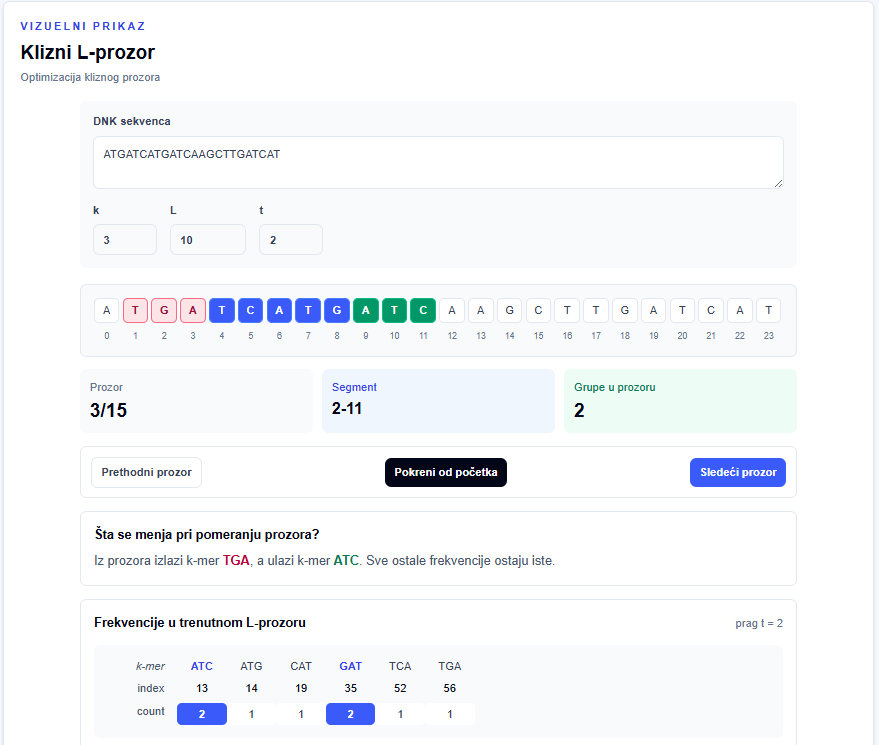
\includegraphics[width=0.75\textwidth]{images/pronalazenje_grupa.png}
\caption{Vizuelizacija optimizovanog pristupa za pronalaženje grupa pomoću kliznog prozora}
\label{fig:pronalazenje_grupa}
\end{figure}

\subsection{\textit{GC-skew }dijagram}

Stranica \textit{GC-skew} dijagram prikazuje algoritam za izračunavanje \textit{GC-skew} vrednosti duž DNK sekvence. Ova vrednost prati razliku između broja baza G i C od početka sekvence do tekuće pozicije. Pozicije na kojima GC-skew funkcija dostiže minimum mogu predstavljati kandidate za početni region replikacije.

Korisnik unosi DNK sekvencu, a aplikacija prikazuje konstrukciju niza vrednosti korak po korak. Vizuelni prikaz obuhvata trenutnu nukleotidnu bazu, trenutnu vrednost funkcije, grafički prikaz \textit{GC-skew} dijagrama i označene pozicije minimuma (Slika \ref{fig:gc_skew}).

\begin{figure}[H]
\centering
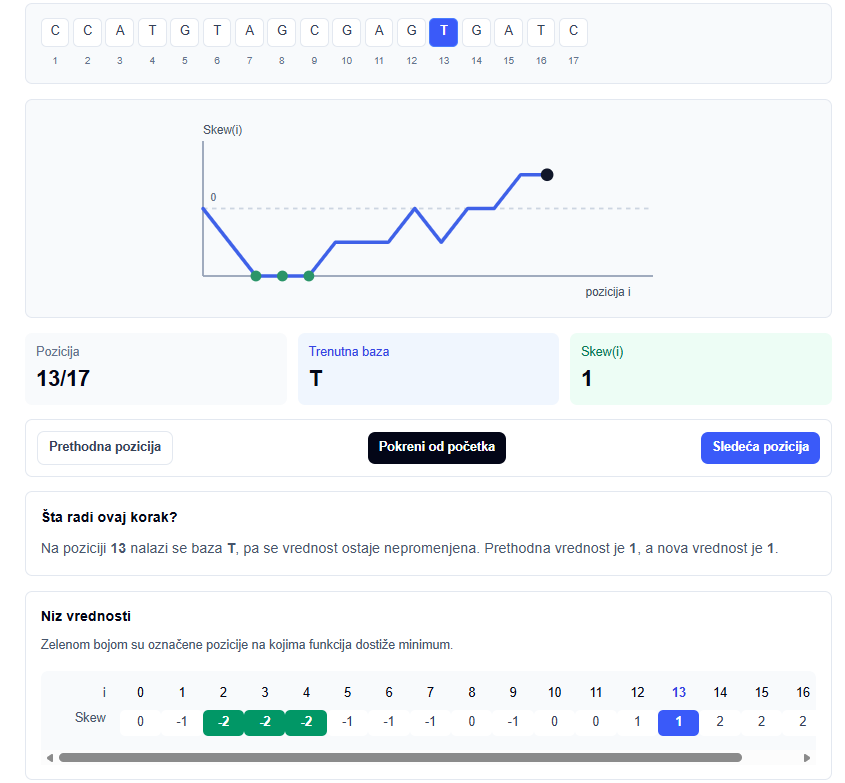
\includegraphics[width=0.75\textwidth]{images/gc_skew_visual.png}
\caption{Vizuelizacija kontrukcije GC-skew dijagrama}
\label{fig:gc_skew}
\end{figure}

\subsection{Približno poklapanje i česte reči sa propustima}

Stranica Propusti obuhvata više povezanih algoritamskih pojmova: Hamingovo rastojanje, približno poklapanje (pod)sekvenci, Hamingovo susedstvo sekvence/k-grama, česte reči sa propustima i obrnute komplemente DNK (pod)sekvenci/k-grama. Ovi pojmovi su važni jer se biološki značajni motivi ne moraju uvek pojaviti u potpuno istom obliku. Mutacije mogu promeniti pojedinačne nukleotide, dok motiv i dalje može zadržati svoju funkciju.

Kao što je prikazano na Slici \ref{fig:hamming}, za Hamingovo rastojanje korisnik unosi dve sekvence iste dužine, a aplikacija prikazuje broj pozicija na kojima se one razlikuju.

\begin{figure}[H]
\centering
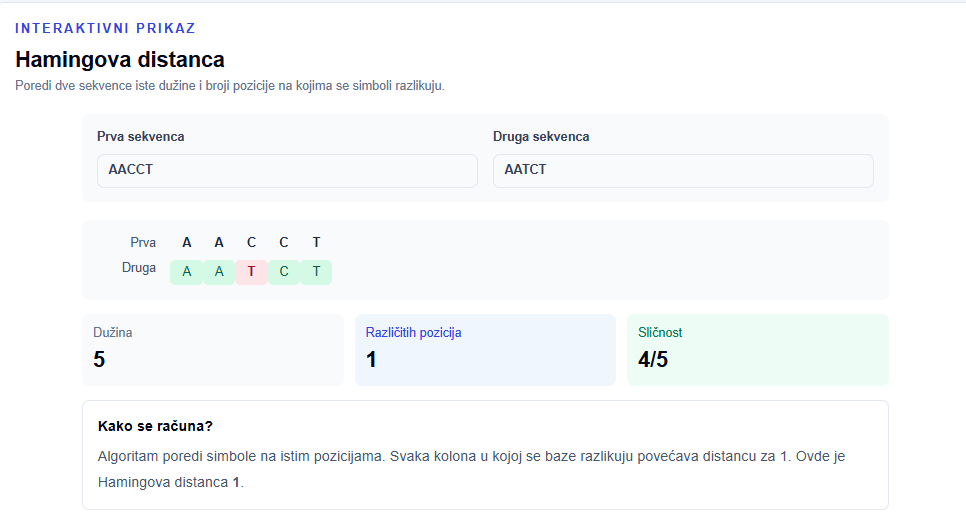
\includegraphics[width=0.75\textwidth]{images/hamming_visual.png}
\caption{Interaktivni prikaz računanja Hamingovog rastojanja za dve sekvence}
\label{fig:hamming}
\end{figure} 

Kod algoritma sa približnim poklapanjima korisnik unosi tekst, obrazac i dozvoljeni broj odstupanja, nakon čega se prikazuju pozicije na kojima se obrazac pojavljuje uz najviše \(d\) razlika. Deo za d-susedstvo prikazuje skup svih sekvenci koje su od zadatog obrasca udaljene najviše \(d\) pozicija (Slika \ref{fig:d}).

\begin{figure}[H]
\centering
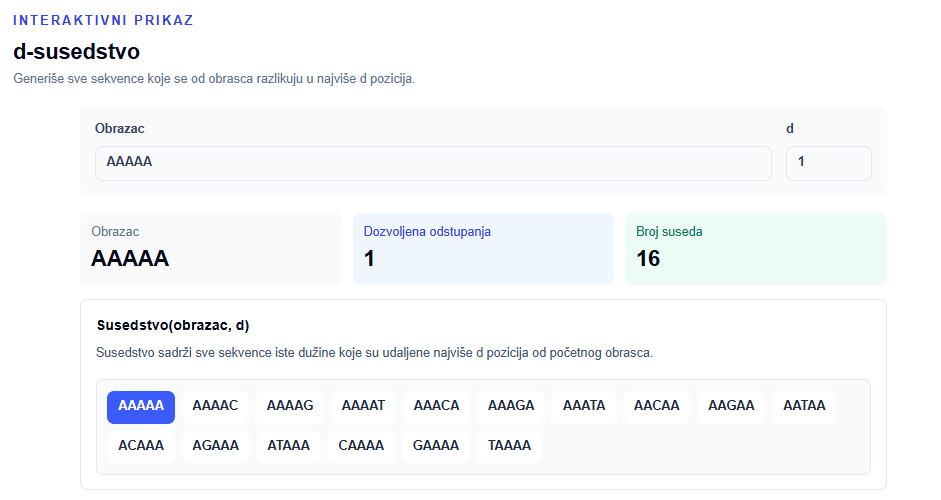
\includegraphics[width=0.75\textwidth]{images/d_susedstvo.png}
\caption{Prikaz d-susedstva niske AAAAA, za d=1}
\label{fig:d}
\end{figure}
 
Na istoj stranici obrađuju se i česte reči sa propustima, gde se traže obrasci koji imaju najveći broj približnih pojavljivanja u tekstu, kao i efikasniji pristup pomoću heš mape. Dodatno, prikazana je i varijanta algoritma koja uzima u obzir obrnute komplemente, što je značajno pri analizi DNK sekvenci jer se motivi mogu posmatrati u obe orijentacije. Na Slici \ref{fig:propusti} vidimo interaktivni prikaz za česte reči sa propustima.

\begin{figure}[H]
\centering
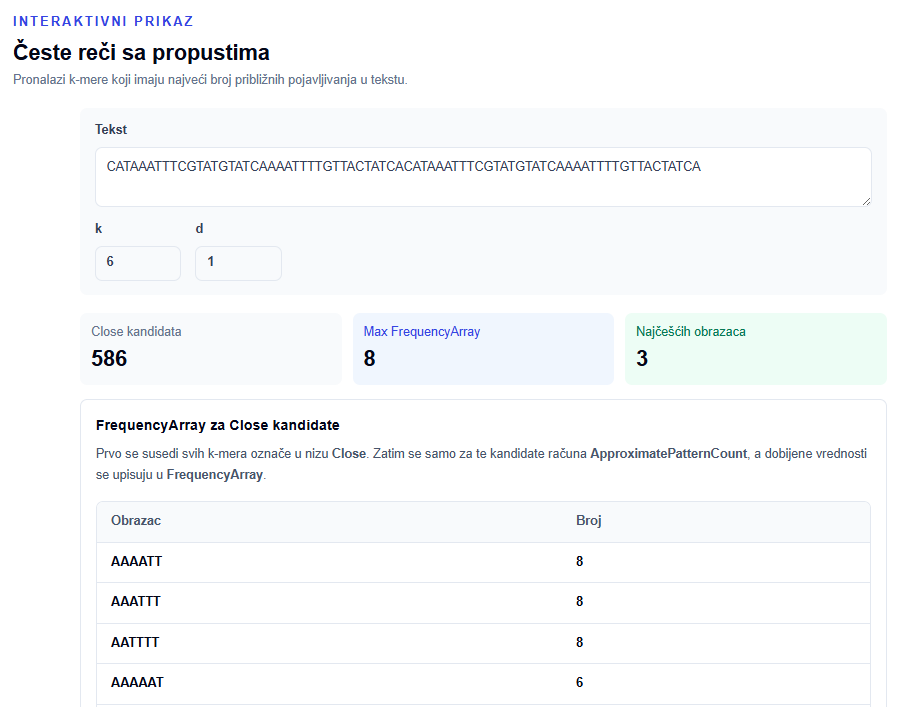
\includegraphics[width=0.75\textwidth]{images/propusti.png}
\caption{Interaktivni prikaz algoritma za  česte reči sa propustima}
\label{fig:propusti}
\end{figure}

\subsection{Literatura}

Stranica Literatura sadrži izvore korišćene za izradu teorijskog i algoritamskog dela lekcije. Pored literature iz oblasti molekularne biologije i bioinformatike, na ovoj stranici nalazi se i link ka \textit{GitHub} repozitorijumu u kojem se nalaze izvorni kod aplikacije, prateći projektni fajlovi i tekstualna verzija rada.


\section{Upotreba alata zasnovanih na veštačkoj inteligenciji}

Tokom izrade ovog rada korišćeni su \textit{Microsoft Copilot} i \textit{ChatGPT} kao pomoćni alati. 
\textit{ChatGPT} korišćen je prvenstveno tokom razvoja programske implementacije, 
za generisanje i unapređenje delova programskog koda, kao i za pomoć pri 
otklanjanju grešaka i pronalaženju odgovarajućih implementacionih rešenja. 
\textit{Microsoft Copilot} je korišćen za doradu, preformulisanje i ujednačavanje stila pojedinih delova teksta.

Sadržaj i predlozi dobijeni korišćenjem alata zasnovanih na veštačkoj inteligenciji nisu preuzimani bez dodatne provere. Ispravnost generisanog i izmenjenog programskog koda proveravana je testiranjem implementiranih funkcionalnosti i poređenjem dobijenih rezultata sa očekivanim rezultatima. Teorijske tvrdnje i objašnjenja proveravani su na osnovu stručne literature navedene u bibliografiji, dok su svi sadržaji uključeni u rad dodatno provereni, korigovani i prilagođeni temi master rada.

% ------------------------------------------------------------------------------
\chapter{Zaključak}
% ------------------------------------------------------------------------------

U ovom radu analizirani su algoritamski pristupi za identifikaciju početnog regiona replikacije u DNK sekvencama. Kroz prikaz različitih algoritama pokazano je na koji način se analiza učestalosti podniski, njihove lokalne raspodele i statističkih karakteristika genoma može iskoristiti za pronalaženje kandidata za \textit{oriC} region.

Za svaki obrađeni algoritam analizirana je osnovna ideja algoritma, složenost, kao i njegove prednosti i ograničenja. Prikazane optimizacije pokazale su kako se odgovarajućim izborom struktura podataka i algoritamskih tehnika može značajno unaprediti efikasnost obrade DNK sekvenci.

Praktični doprinos ovog rada predstavlja razvoj elektronske lekcije koja objedinjuje teorijska objašnjenja obrađenih algoritama i njihovu interaktivnu primenu kroz veb aplikaciju. Implementirana aplikacija omogućava korisnicima da pokreću algoritme nad proizvoljnim ulaznim podacima, prate njihovo izvršavanje korak po korak i analiziraju dobijene rezultate, čime se olakšava razumevanje njihovog rada i primene u bioinformatici.

Iako opisani algoritmi predstavljaju značajnu osnovu za identifikaciju početnog regiona replikacije, u praksi se oni često kombinuju sa drugim bioinformatičkim metodama i biološkim informacijama kako bi se postigla veća pouzdanost rezultata. Budući razvoj može obuhvatiti proširenje elektronske lekcije novim algoritmima i interaktivnim primerima, kao i primenu opisanih metoda na većim skupovima realnih genomskih podataka, čime bi se dodatno unapredila njena obrazovna i praktična vrednost.
% ------------------------------------------------------------------------------
% Literatura
% ------------------------------------------------------------------------------
\literatura

% ==============================================================================
% Završni deo teze i prilozi
\backmatter
% ==============================================================================

% ------------------------------------------------------------------------------
% Biografija kandidata
\begin{biografija}
  \textbf{Dunja Čitlučanin} rođena je 22. septembra 1998. godine u Beogradu. Smer Računarstvo i informatika na Matematičkom fakultetu Univerziteta u Beogradu upisala je 2017. godine, a završila 2022. godine. Nakon toga je upisala master studije na istom smeru. 
  Od 2023. do novembra 2024. godine je zaposlena na poziciji \emph{Junior Software engineer}  u firmi \textbf{Telekom Srbija}, a potom od novembra 2024. godine do marta 2026. je zaposlena na poziciji \emph{Software developer} u firmi \textbf{Development and Testing Center}. Sada je zaposlena kao \emph{Data scientist} u firmi \textbf{NCR Atleos}. 
\end{biografija}
\end{document}